\documentclass[a4paper]{book}
\usepackage{makeidx}
\usepackage{natbib}
\usepackage{graphicx}
\usepackage{multicol}
\usepackage{float}
\usepackage{listings}
\usepackage{color}
\usepackage{ifthen}
\usepackage[table]{xcolor}
\usepackage{textcomp}
\usepackage{alltt}
\usepackage{ifpdf}
\ifpdf
\usepackage[pdftex,
            pagebackref=true,
            colorlinks=true,
            linkcolor=blue,
            unicode
           ]{hyperref}
\else
\usepackage[ps2pdf,
            pagebackref=true,
            colorlinks=true,
            linkcolor=blue,
            unicode
           ]{hyperref}
\usepackage{pspicture}
\fi
\usepackage[utf8]{inputenc}
\usepackage[spanish]{babel}
\usepackage{mathptmx}
\usepackage[scaled=.90]{helvet}
\usepackage{courier}
\usepackage{sectsty}
\usepackage[titles]{tocloft}
\usepackage{doxygen}
\lstset{language=C++,inputencoding=utf8,basicstyle=\footnotesize,breaklines=true,breakatwhitespace=true,tabsize=4,numbers=left }
\makeindex
\setcounter{tocdepth}{3}
\renewcommand{\footrulewidth}{0.4pt}
\renewcommand{\familydefault}{\sfdefault}
\hfuzz=15pt
\setlength{\emergencystretch}{15pt}
\hbadness=750
\tolerance=750
\begin{document}
\hypersetup{pageanchor=false,citecolor=blue}
\begin{titlepage}
\vspace*{7cm}
\begin{center}
{\Large \-Social\-Book \\[1ex]\large 0.\-1 }\\
\vspace*{1cm}
{\large \-Generado por Doxygen 1.7.6.1}\\
\vspace*{0.5cm}
{\small Martes, 9 de Mayo de 2017 02:03:52}\\
\end{center}
\end{titlepage}
\clearemptydoublepage
\pagenumbering{roman}
\tableofcontents
\clearemptydoublepage
\pagenumbering{arabic}
\hypersetup{pageanchor=true,citecolor=blue}
\chapter{\-Indice de namespaces}
\section{\-Lista de 'namespaces'}
\-Lista de toda la documentación de los 'namespaces', con una breve descripción\-:\begin{DoxyCompactList}
\item\contentsline{section}{\hyperlink{namespace_laravel}{\-Laravel} }{\pageref{namespace_laravel}}{}
\end{DoxyCompactList}

\chapter{Índice de estructura de datos}
\section{\-Jerarquía de la clase}
\-Esta lista de herencias esta ordenada aproximadamente por orden alfabético\-:\begin{DoxyCompactList}
\item \contentsline{section}{\-Agregar\-Campo\-Booleano\-Superuser\-Tabla\-User}{\pageref{class_agregar_campo_booleano_superuser_tabla_user}}{}
\item \contentsline{section}{\-Agregar\-Campo\-Rut\-Inst\-A\-User}{\pageref{class_agregar_campo_rut_inst_a_user}}{}
\item \contentsline{section}{\-Aviso}{\pageref{class_app_1_1_aviso}}{}
\item \contentsline{section}{\-Aviso\-Table\-Seeder}{\pageref{class_aviso_table_seeder}}{}
\item \contentsline{section}{\-Controller}{\pageref{class_app_1_1_http_1_1_controllers_1_1_controller}}{}
\begin{DoxyCompactList}
\item \contentsline{section}{\-Auth\-Controller}{\pageref{class_app_1_1_http_1_1_controllers_1_1_auth_1_1_auth_controller}}{}
\item \contentsline{section}{\-Password\-Controller}{\pageref{class_app_1_1_http_1_1_controllers_1_1_auth_1_1_password_controller}}{}
\item \contentsline{section}{\-Home\-Controller}{\pageref{class_app_1_1_http_1_1_controllers_1_1_home_controller}}{}
\item \contentsline{section}{\-Homepage\-Controller}{\pageref{class_app_1_1_http_1_1_controllers_1_1_homepage_controller}}{}
\item \contentsline{section}{\-Institucion\-Controller}{\pageref{class_app_1_1_http_1_1_controllers_1_1_institucion_controller}}{}
\end{DoxyCompactList}
\item \contentsline{section}{\-Crear\-Tabla\-Aviso}{\pageref{class_crear_tabla_aviso}}{}
\item \contentsline{section}{\-Crear\-Tabla\-Institucion}{\pageref{class_crear_tabla_institucion}}{}
\item \contentsline{section}{\-Create\-Password\-Resets\-Table}{\pageref{class_create_password_resets_table}}{}
\item \contentsline{section}{\-Create\-Users\-Table}{\pageref{class_create_users_table}}{}
\item \contentsline{section}{\-Database\-Seeder}{\pageref{class_database_seeder}}{}
\item \contentsline{section}{\-Institucion}{\pageref{class_app_1_1_institucion}}{}
\item \contentsline{section}{\-Institucion\-Table\-Seeder}{\pageref{class_institucion_table_seeder}}{}
\item \contentsline{section}{\-Test\-Case}{\pageref{class_test_case}}{}
\begin{DoxyCompactList}
\item \contentsline{section}{\-Example\-Test}{\pageref{class_example_test}}{}
\item \contentsline{section}{\-Ver\-Instituciones\-Test}{\pageref{class_ver_instituciones_test}}{}
\end{DoxyCompactList}
\item \contentsline{section}{\-User}{\pageref{class_app_1_1_user}}{}
\item \contentsline{section}{\-User\-Table\-Seeder}{\pageref{class_user_table_seeder}}{}
\end{DoxyCompactList}

\chapter{Índice de estructura de datos}
\section{\-Estructura de datos}
\-Lista de estructuras con una breve descripción\-:\begin{DoxyCompactList}
\item\contentsline{section}{\hyperlink{class_agregar_campo_booleano_superuser_tabla_user}{\-Agregar\-Campo\-Booleano\-Superuser\-Tabla\-User} }{\pageref{class_agregar_campo_booleano_superuser_tabla_user}}{}
\item\contentsline{section}{\hyperlink{class_agregar_campo_rut_inst_a_user}{\-Agregar\-Campo\-Rut\-Inst\-A\-User} }{\pageref{class_agregar_campo_rut_inst_a_user}}{}
\item\contentsline{section}{\hyperlink{class_app_1_1_http_1_1_controllers_1_1_auth_1_1_auth_controller}{\-Auth\-Controller} }{\pageref{class_app_1_1_http_1_1_controllers_1_1_auth_1_1_auth_controller}}{}
\item\contentsline{section}{\hyperlink{class_app_1_1_aviso}{\-Aviso} }{\pageref{class_app_1_1_aviso}}{}
\item\contentsline{section}{\hyperlink{class_aviso_table_seeder}{\-Aviso\-Table\-Seeder} }{\pageref{class_aviso_table_seeder}}{}
\item\contentsline{section}{\hyperlink{class_app_1_1_http_1_1_controllers_1_1_contact_controller}{\-Contact\-Controller} }{\pageref{class_app_1_1_http_1_1_controllers_1_1_contact_controller}}{}
\item\contentsline{section}{\hyperlink{class_app_1_1_http_1_1_controllers_1_1_controller}{\-Controller} }{\pageref{class_app_1_1_http_1_1_controllers_1_1_controller}}{}
\item\contentsline{section}{\hyperlink{class_crear_tabla_aviso}{\-Crear\-Tabla\-Aviso} }{\pageref{class_crear_tabla_aviso}}{}
\item\contentsline{section}{\hyperlink{class_crear_tabla_institucion}{\-Crear\-Tabla\-Institucion} }{\pageref{class_crear_tabla_institucion}}{}
\item\contentsline{section}{\hyperlink{class_create_password_resets_table}{\-Create\-Password\-Resets\-Table} }{\pageref{class_create_password_resets_table}}{}
\item\contentsline{section}{\hyperlink{class_create_roles_table}{\-Create\-Roles\-Table} }{\pageref{class_create_roles_table}}{}
\item\contentsline{section}{\hyperlink{class_create_user_roles_table}{\-Create\-User\-Roles\-Table} }{\pageref{class_create_user_roles_table}}{}
\item\contentsline{section}{\hyperlink{class_create_users_table}{\-Create\-Users\-Table} }{\pageref{class_create_users_table}}{}
\item\contentsline{section}{\hyperlink{class_database_seeder}{\-Database\-Seeder} }{\pageref{class_database_seeder}}{}
\item\contentsline{section}{\hyperlink{class_example_test}{\-Example\-Test} }{\pageref{class_example_test}}{}
\item\contentsline{section}{\hyperlink{class_app_1_1_http_1_1_controllers_1_1_home_controller}{\-Home\-Controller} }{\pageref{class_app_1_1_http_1_1_controllers_1_1_home_controller}}{}
\item\contentsline{section}{\hyperlink{class_app_1_1_http_1_1_controllers_1_1_homepage_controller}{\-Homepage\-Controller} }{\pageref{class_app_1_1_http_1_1_controllers_1_1_homepage_controller}}{}
\item\contentsline{section}{\hyperlink{class_app_1_1_imagen}{\-Imagen} }{\pageref{class_app_1_1_imagen}}{}
\item\contentsline{section}{\hyperlink{class_imagen_aviso}{\-Imagen\-Aviso} }{\pageref{class_imagen_aviso}}{}
\item\contentsline{section}{\hyperlink{class_app_1_1_imagen_evento}{\-Imagen\-Evento} }{\pageref{class_app_1_1_imagen_evento}}{}
\item\contentsline{section}{\hyperlink{class_imagen_table_seeder}{\-Imagen\-Table\-Seeder} }{\pageref{class_imagen_table_seeder}}{}
\item\contentsline{section}{\hyperlink{class_app_1_1_institucion}{\-Institucion} }{\pageref{class_app_1_1_institucion}}{}
\item\contentsline{section}{\hyperlink{class_app_1_1_http_1_1_controllers_1_1_institucion_controller}{\-Institucion\-Controller} }{\pageref{class_app_1_1_http_1_1_controllers_1_1_institucion_controller}}{}
\item\contentsline{section}{\hyperlink{class_institucion_table_seeder}{\-Institucion\-Table\-Seeder} }{\pageref{class_institucion_table_seeder}}{}
\item\contentsline{section}{\hyperlink{class_app_1_1_noticia}{\-Noticia} }{\pageref{class_app_1_1_noticia}}{}
\item\contentsline{section}{\hyperlink{class_app_1_1_http_1_1_controllers_1_1_auth_1_1_password_controller}{\-Password\-Controller} }{\pageref{class_app_1_1_http_1_1_controllers_1_1_auth_1_1_password_controller}}{}
\item\contentsline{section}{\hyperlink{class_app_1_1_role}{\-Role} }{\pageref{class_app_1_1_role}}{}
\item\contentsline{section}{\hyperlink{class_roles_table_seeder}{\-Roles\-Table\-Seeder} }{\pageref{class_roles_table_seeder}}{}
\item\contentsline{section}{\hyperlink{class_app_1_1_http_1_1_controllers_1_1_storage_controller}{\-Storage\-Controller} }{\pageref{class_app_1_1_http_1_1_controllers_1_1_storage_controller}}{}
\item\contentsline{section}{\hyperlink{class_tabla_imagen}{\-Tabla\-Imagen} }{\pageref{class_tabla_imagen}}{}
\item\contentsline{section}{\hyperlink{class_tabla_imagen_evento}{\-Tabla\-Imagen\-Evento} }{\pageref{class_tabla_imagen_evento}}{}
\item\contentsline{section}{\hyperlink{class_tabla_noticia}{\-Tabla\-Noticia} }{\pageref{class_tabla_noticia}}{}
\item\contentsline{section}{\hyperlink{class_test_case}{\-Test\-Case} }{\pageref{class_test_case}}{}
\item\contentsline{section}{\hyperlink{class_app_1_1_user}{\-User} }{\pageref{class_app_1_1_user}}{}
\item\contentsline{section}{\hyperlink{class_user_table_seeder}{\-User\-Table\-Seeder} }{\pageref{class_user_table_seeder}}{}
\item\contentsline{section}{\hyperlink{class_ver_instituciones_test}{\-Ver\-Instituciones\-Test} }{\pageref{class_ver_instituciones_test}}{}
\end{DoxyCompactList}

\chapter{\-Documentación de namespaces}
\hypertarget{namespace_laravel}{\section{\-Referencia del \-Namespace \-Laravel}
\label{namespace_laravel}\index{\-Laravel@{\-Laravel}}
}


\subsection{\-Descripción detallada}
\hyperlink{namespace_laravel}{\-Laravel} -\/ \-A \-P\-H\-P \-Framework \-For \-Web \-Artisans

\begin{DoxyAuthor}{\-Autor}
\-Taylor \-Otwell $<$\href{mailto:taylorotwell@gmail.com}{\tt taylorotwell@gmail.\-com}$>$ 
\end{DoxyAuthor}

\chapter{\-Documentación de las estructuras de datos}
\hypertarget{class_agregar_campo_booleano_superuser_tabla_user}{\section{\-Referencia de la \-Clase \-Agregar\-Campo\-Booleano\-Superuser\-Tabla\-User}
\label{class_agregar_campo_booleano_superuser_tabla_user}\index{\-Agregar\-Campo\-Booleano\-Superuser\-Tabla\-User@{\-Agregar\-Campo\-Booleano\-Superuser\-Tabla\-User}}
}
\subsection*{\-Métodos públicos}
\begin{DoxyCompactItemize}
\item 
\hyperlink{class_agregar_campo_booleano_superuser_tabla_user_a4edef5efd5ab94ce9d17295898ead93a}{up} ()
\item 
\hyperlink{class_agregar_campo_booleano_superuser_tabla_user_af5fda92f47a449c7a33f9dd5ef5aa6c3}{down} ()
\end{DoxyCompactItemize}


\subsection{\-Documentación de las funciones miembro}
\hypertarget{class_agregar_campo_booleano_superuser_tabla_user_af5fda92f47a449c7a33f9dd5ef5aa6c3}{\index{\-Agregar\-Campo\-Booleano\-Superuser\-Tabla\-User@{\-Agregar\-Campo\-Booleano\-Superuser\-Tabla\-User}!down@{down}}
\index{down@{down}!AgregarCampoBooleanoSuperuserTablaUser@{\-Agregar\-Campo\-Booleano\-Superuser\-Tabla\-User}}
\subsubsection[{down}]{\setlength{\rightskip}{0pt plus 5cm}{\bf down} (
\begin{DoxyParamCaption}
{}
\end{DoxyParamCaption}
)}}\label{class_agregar_campo_booleano_superuser_tabla_user_af5fda92f47a449c7a33f9dd5ef5aa6c3}
\-Reverse the migrations.

\begin{DoxyReturn}{\-Devuelve}
void 
\end{DoxyReturn}
\hypertarget{class_agregar_campo_booleano_superuser_tabla_user_a4edef5efd5ab94ce9d17295898ead93a}{\index{\-Agregar\-Campo\-Booleano\-Superuser\-Tabla\-User@{\-Agregar\-Campo\-Booleano\-Superuser\-Tabla\-User}!up@{up}}
\index{up@{up}!AgregarCampoBooleanoSuperuserTablaUser@{\-Agregar\-Campo\-Booleano\-Superuser\-Tabla\-User}}
\subsubsection[{up}]{\setlength{\rightskip}{0pt plus 5cm}{\bf up} (
\begin{DoxyParamCaption}
{}
\end{DoxyParamCaption}
)}}\label{class_agregar_campo_booleano_superuser_tabla_user_a4edef5efd5ab94ce9d17295898ead93a}
\-Run the migrations.

\begin{DoxyReturn}{\-Devuelve}
void 
\end{DoxyReturn}


\-La documentación para esta clase fue generada a partir del siguiente fichero\-:\begin{DoxyCompactItemize}
\item 
/home/travis/build/tvargasvicencio/ayudalab/database/migrations/2016\-\_\-12\-\_\-26\-\_\-184042\-\_\-agregar\-\_\-campo\-\_\-booleano\-\_\-superuser\-\_\-tabla\-\_\-user.\-php\end{DoxyCompactItemize}

\hypertarget{class_agregar_campo_rut_inst_a_user}{\section{\-Referencia de la \-Clase \-Agregar\-Campo\-Rut\-Inst\-A\-User}
\label{class_agregar_campo_rut_inst_a_user}\index{\-Agregar\-Campo\-Rut\-Inst\-A\-User@{\-Agregar\-Campo\-Rut\-Inst\-A\-User}}
}
\subsection*{\-Métodos públicos}
\begin{DoxyCompactItemize}
\item 
\hyperlink{class_agregar_campo_rut_inst_a_user_a4edef5efd5ab94ce9d17295898ead93a}{up} ()
\item 
\hyperlink{class_agregar_campo_rut_inst_a_user_af5fda92f47a449c7a33f9dd5ef5aa6c3}{down} ()
\end{DoxyCompactItemize}


\subsection{\-Documentación de las funciones miembro}
\hypertarget{class_agregar_campo_rut_inst_a_user_af5fda92f47a449c7a33f9dd5ef5aa6c3}{\index{\-Agregar\-Campo\-Rut\-Inst\-A\-User@{\-Agregar\-Campo\-Rut\-Inst\-A\-User}!down@{down}}
\index{down@{down}!AgregarCampoRutInstAUser@{\-Agregar\-Campo\-Rut\-Inst\-A\-User}}
\subsubsection[{down}]{\setlength{\rightskip}{0pt plus 5cm}{\bf down} (
\begin{DoxyParamCaption}
{}
\end{DoxyParamCaption}
)}}\label{class_agregar_campo_rut_inst_a_user_af5fda92f47a449c7a33f9dd5ef5aa6c3}
\-Reverse the migrations.

\begin{DoxyReturn}{\-Devuelve}
void 
\end{DoxyReturn}
\hypertarget{class_agregar_campo_rut_inst_a_user_a4edef5efd5ab94ce9d17295898ead93a}{\index{\-Agregar\-Campo\-Rut\-Inst\-A\-User@{\-Agregar\-Campo\-Rut\-Inst\-A\-User}!up@{up}}
\index{up@{up}!AgregarCampoRutInstAUser@{\-Agregar\-Campo\-Rut\-Inst\-A\-User}}
\subsubsection[{up}]{\setlength{\rightskip}{0pt plus 5cm}{\bf up} (
\begin{DoxyParamCaption}
{}
\end{DoxyParamCaption}
)}}\label{class_agregar_campo_rut_inst_a_user_a4edef5efd5ab94ce9d17295898ead93a}
\-Run the migrations.

\begin{DoxyReturn}{\-Devuelve}
void 
\end{DoxyReturn}


\-La documentación para esta clase fue generada a partir del siguiente fichero\-:\begin{DoxyCompactItemize}
\item 
/home/travis/build/tvargasvicencio/ayudalab/database/migrations/2016\-\_\-12\-\_\-23\-\_\-025721\-\_\-agregar\-\_\-campo\-\_\-rut\-\_\-inst\-\_\-a\-\_\-user.\-php\end{DoxyCompactItemize}

\hypertarget{class_app_1_1_http_1_1_controllers_1_1_auth_1_1_auth_controller}{\section{\-Referencia de la \-Clase \-Auth\-Controller}
\label{class_app_1_1_http_1_1_controllers_1_1_auth_1_1_auth_controller}\index{\-Auth\-Controller@{\-Auth\-Controller}}
}


\-Diagrama de herencias de \-Auth\-Controller
\nopagebreak
\begin{figure}[H]
\begin{center}
\leavevmode
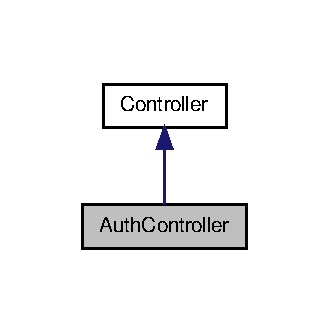
\includegraphics[width=158pt]{class_app_1_1_http_1_1_controllers_1_1_auth_1_1_auth_controller__inherit__graph}
\end{center}
\end{figure}


\-Diagrama de colaboración para \-Auth\-Controller\-:
\nopagebreak
\begin{figure}[H]
\begin{center}
\leavevmode
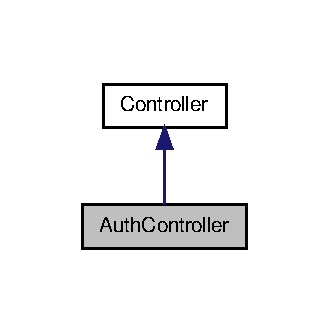
\includegraphics[width=158pt]{class_app_1_1_http_1_1_controllers_1_1_auth_1_1_auth_controller__coll__graph}
\end{center}
\end{figure}
\subsection*{\-Métodos públicos}
\begin{DoxyCompactItemize}
\item 
\hyperlink{class_app_1_1_http_1_1_controllers_1_1_auth_1_1_auth_controller_a095c5d389db211932136b53f25f39685}{\-\_\-\-\_\-construct} ()
\end{DoxyCompactItemize}
\subsection*{\-Métodos protegidos}
\begin{DoxyCompactItemize}
\item 
\hyperlink{class_app_1_1_http_1_1_controllers_1_1_auth_1_1_auth_controller_aa47350de63ea5295d9c9718e3d09135c}{validator} (array \$data)
\item 
\hyperlink{class_app_1_1_http_1_1_controllers_1_1_auth_1_1_auth_controller_a791ba6c150a0a3047c7d8735e62cad02}{create} (array \$data)
\end{DoxyCompactItemize}
\subsection*{\-Atributos protegidos}
\begin{DoxyCompactItemize}
\item 
\hypertarget{class_app_1_1_http_1_1_controllers_1_1_auth_1_1_auth_controller_a1d19101ee5de7186666ce86a530cd501}{{\bfseries \$redirect\-To} = '/dashboard/informacion\-Institucional'}\label{class_app_1_1_http_1_1_controllers_1_1_auth_1_1_auth_controller_a1d19101ee5de7186666ce86a530cd501}

\end{DoxyCompactItemize}


\subsection{\-Documentación del constructor y destructor}
\hypertarget{class_app_1_1_http_1_1_controllers_1_1_auth_1_1_auth_controller_a095c5d389db211932136b53f25f39685}{\index{\-App\-::\-Http\-::\-Controllers\-::\-Auth\-::\-Auth\-Controller@{\-App\-::\-Http\-::\-Controllers\-::\-Auth\-::\-Auth\-Controller}!\-\_\-\-\_\-construct@{\-\_\-\-\_\-construct}}
\index{\-\_\-\-\_\-construct@{\-\_\-\-\_\-construct}!App::Http::Controllers::Auth::AuthController@{\-App\-::\-Http\-::\-Controllers\-::\-Auth\-::\-Auth\-Controller}}
\subsubsection[{\-\_\-\-\_\-construct}]{\setlength{\rightskip}{0pt plus 5cm}{\bf \-\_\-\-\_\-construct} (
\begin{DoxyParamCaption}
{}
\end{DoxyParamCaption}
)}}\label{class_app_1_1_http_1_1_controllers_1_1_auth_1_1_auth_controller_a095c5d389db211932136b53f25f39685}
\-Create a new authentication controller instance.

\begin{DoxyReturn}{\-Devuelve}
void 
\end{DoxyReturn}


\subsection{\-Documentación de las funciones miembro}
\hypertarget{class_app_1_1_http_1_1_controllers_1_1_auth_1_1_auth_controller_a791ba6c150a0a3047c7d8735e62cad02}{\index{\-App\-::\-Http\-::\-Controllers\-::\-Auth\-::\-Auth\-Controller@{\-App\-::\-Http\-::\-Controllers\-::\-Auth\-::\-Auth\-Controller}!create@{create}}
\index{create@{create}!App::Http::Controllers::Auth::AuthController@{\-App\-::\-Http\-::\-Controllers\-::\-Auth\-::\-Auth\-Controller}}
\subsubsection[{create}]{\setlength{\rightskip}{0pt plus 5cm}{\bf create} (
\begin{DoxyParamCaption}
\item[{array \$}]{data}
\end{DoxyParamCaption}
)\hspace{0.3cm}{\ttfamily  \mbox{[}protected\mbox{]}}}}\label{class_app_1_1_http_1_1_controllers_1_1_auth_1_1_auth_controller_a791ba6c150a0a3047c7d8735e62cad02}
\-Create a new user instance after a valid registration.


\begin{DoxyParams}[1]{\-Parámetros}
array & {\em \$data} & \\
\hline
\end{DoxyParams}
\begin{DoxyReturn}{\-Devuelve}
\hyperlink{class_app_1_1_user}{\-User} 
\end{DoxyReturn}
\hypertarget{class_app_1_1_http_1_1_controllers_1_1_auth_1_1_auth_controller_aa47350de63ea5295d9c9718e3d09135c}{\index{\-App\-::\-Http\-::\-Controllers\-::\-Auth\-::\-Auth\-Controller@{\-App\-::\-Http\-::\-Controllers\-::\-Auth\-::\-Auth\-Controller}!validator@{validator}}
\index{validator@{validator}!App::Http::Controllers::Auth::AuthController@{\-App\-::\-Http\-::\-Controllers\-::\-Auth\-::\-Auth\-Controller}}
\subsubsection[{validator}]{\setlength{\rightskip}{0pt plus 5cm}{\bf validator} (
\begin{DoxyParamCaption}
\item[{array \$}]{data}
\end{DoxyParamCaption}
)\hspace{0.3cm}{\ttfamily  \mbox{[}protected\mbox{]}}}}\label{class_app_1_1_http_1_1_controllers_1_1_auth_1_1_auth_controller_aa47350de63ea5295d9c9718e3d09135c}
\-Get a validator for an incoming registration request.


\begin{DoxyParams}[1]{\-Parámetros}
array & {\em \$data} & \\
\hline
\end{DoxyParams}
\begin{DoxyReturn}{\-Devuelve}

\end{DoxyReturn}


\-La documentación para esta clase fue generada a partir del siguiente fichero\-:\begin{DoxyCompactItemize}
\item 
/home/travis/build/tvargasvicencio/ayudalab/app/\-Http/\-Controllers/\-Auth/\-Auth\-Controller.\-php\end{DoxyCompactItemize}

\hypertarget{class_app_1_1_aviso}{\section{\-Referencia de la \-Clase \-Aviso}
\label{class_app_1_1_aviso}\index{\-Aviso@{\-Aviso}}
}
\subsection*{\-Métodos públicos}
\begin{DoxyCompactItemize}
\item 
\hyperlink{class_app_1_1_aviso_abfb0e179daf0a8f710adbb1456e5b3eb}{institucion} ()
\item 
\hyperlink{class_app_1_1_aviso_ae8a275690ff1b618e1947378b0ed73ae}{user} ()
\end{DoxyCompactItemize}
\subsection*{\-Atributos protegidos}
\begin{DoxyCompactItemize}
\item 
\hypertarget{class_app_1_1_aviso_ae8876a14058f368335baccf35af4a22b}{{\bfseries \$table} = 'aviso'}\label{class_app_1_1_aviso_ae8876a14058f368335baccf35af4a22b}

\item 
\hypertarget{class_app_1_1_aviso_a6a90e74ccdf5efd70d51d10c906f8e32}{{\bfseries \$fillable} = \mbox{[}'descripcion', 'titulo', 'img', 'rut\-\_\-inst', 'user\-\_\-id'\mbox{]}}\label{class_app_1_1_aviso_a6a90e74ccdf5efd70d51d10c906f8e32}

\end{DoxyCompactItemize}


\subsection{\-Documentación de las funciones miembro}
\hypertarget{class_app_1_1_aviso_abfb0e179daf0a8f710adbb1456e5b3eb}{\index{\-App\-::\-Aviso@{\-App\-::\-Aviso}!institucion@{institucion}}
\index{institucion@{institucion}!App::Aviso@{\-App\-::\-Aviso}}
\subsubsection[{institucion}]{\setlength{\rightskip}{0pt plus 5cm}{\bf institucion} (
\begin{DoxyParamCaption}
{}
\end{DoxyParamCaption}
)}}\label{class_app_1_1_aviso_abfb0e179daf0a8f710adbb1456e5b3eb}
\-Indica que un \hyperlink{class_app_1_1_aviso}{\-Aviso} pertenece a una \hyperlink{class_app_1_1_institucion}{\-Institucion}

\begin{DoxyReturn}{\-Devuelve}
$<$type$>$ ( description\-\_\-of\-\_\-the\-\_\-return\-\_\-value ) 
\end{DoxyReturn}
\hypertarget{class_app_1_1_aviso_ae8a275690ff1b618e1947378b0ed73ae}{\index{\-App\-::\-Aviso@{\-App\-::\-Aviso}!user@{user}}
\index{user@{user}!App::Aviso@{\-App\-::\-Aviso}}
\subsubsection[{user}]{\setlength{\rightskip}{0pt plus 5cm}{\bf user} (
\begin{DoxyParamCaption}
{}
\end{DoxyParamCaption}
)}}\label{class_app_1_1_aviso_ae8a275690ff1b618e1947378b0ed73ae}
\-Indica que un \hyperlink{class_app_1_1_aviso}{\-Aviso} pertenece a un \hyperlink{class_app_1_1_user}{\-User}

\begin{DoxyReturn}{\-Devuelve}
$<$type$>$ ( description\-\_\-of\-\_\-the\-\_\-return\-\_\-value ) 
\end{DoxyReturn}


\-La documentación para esta clase fue generada a partir del siguiente fichero\-:\begin{DoxyCompactItemize}
\item 
/home/travis/build/tvargasvicencio/ayudalab/app/\-Aviso.\-php\end{DoxyCompactItemize}

\hypertarget{class_aviso_table_seeder}{\section{\-Referencia de la \-Clase \-Aviso\-Table\-Seeder}
\label{class_aviso_table_seeder}\index{\-Aviso\-Table\-Seeder@{\-Aviso\-Table\-Seeder}}
}
\subsection*{\-Métodos públicos}
\begin{DoxyCompactItemize}
\item 
\hyperlink{class_aviso_table_seeder_afb0fafe7e02a3ae1993c01c19fad2bae}{run} ()
\end{DoxyCompactItemize}


\subsection{\-Documentación de las funciones miembro}
\hypertarget{class_aviso_table_seeder_afb0fafe7e02a3ae1993c01c19fad2bae}{\index{\-Aviso\-Table\-Seeder@{\-Aviso\-Table\-Seeder}!run@{run}}
\index{run@{run}!AvisoTableSeeder@{\-Aviso\-Table\-Seeder}}
\subsubsection[{run}]{\setlength{\rightskip}{0pt plus 5cm}{\bf run} (
\begin{DoxyParamCaption}
{}
\end{DoxyParamCaption}
)}}\label{class_aviso_table_seeder_afb0fafe7e02a3ae1993c01c19fad2bae}
\-Run the database seeds.

\begin{DoxyReturn}{\-Devuelve}
void 
\end{DoxyReturn}


\-La documentación para esta clase fue generada a partir del siguiente fichero\-:\begin{DoxyCompactItemize}
\item 
/home/travis/build/tvargasvicencio/ayudalab/database/seeds/\-Aviso\-Table\-Seeder.\-php\end{DoxyCompactItemize}

\hypertarget{class_app_1_1_http_1_1_controllers_1_1_contact_controller}{\section{\-Referencia de la \-Clase \-Contact\-Controller}
\label{class_app_1_1_http_1_1_controllers_1_1_contact_controller}\index{\-Contact\-Controller@{\-Contact\-Controller}}
}


\-Diagrama de herencias de \-Contact\-Controller
\nopagebreak
\begin{figure}[H]
\begin{center}
\leavevmode
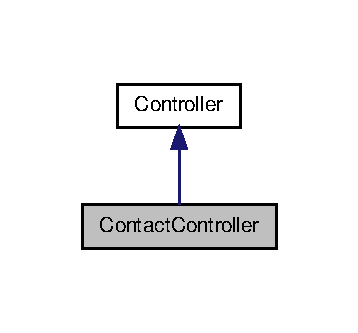
\includegraphics[width=172pt]{class_app_1_1_http_1_1_controllers_1_1_contact_controller__inherit__graph}
\end{center}
\end{figure}


\-Diagrama de colaboración para \-Contact\-Controller\-:
\nopagebreak
\begin{figure}[H]
\begin{center}
\leavevmode
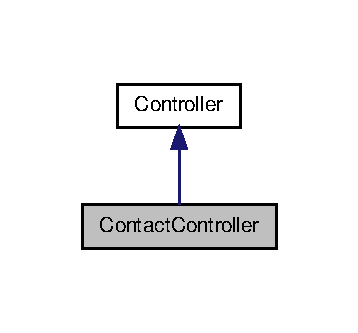
\includegraphics[width=172pt]{class_app_1_1_http_1_1_controllers_1_1_contact_controller__coll__graph}
\end{center}
\end{figure}
\subsection*{\-Métodos públicos}
\begin{DoxyCompactItemize}
\item 
\hypertarget{class_app_1_1_http_1_1_controllers_1_1_contact_controller_a149eb92716c1084a935e04a8d95f7347}{{\bfseries index} ()}\label{class_app_1_1_http_1_1_controllers_1_1_contact_controller_a149eb92716c1084a935e04a8d95f7347}

\end{DoxyCompactItemize}


\-La documentación para esta clase fue generada a partir del siguiente fichero\-:\begin{DoxyCompactItemize}
\item 
/home/travis/build/tvargasvicencio/ayudalab/app/\-Http/\-Controllers/\-Contact\-Controller.\-php\end{DoxyCompactItemize}

\hypertarget{class_app_1_1_http_1_1_controllers_1_1_controller}{\section{\-Referencia de la \-Clase \-Controller}
\label{class_app_1_1_http_1_1_controllers_1_1_controller}\index{\-Controller@{\-Controller}}
}


\-Diagrama de herencias de \-Controller
\nopagebreak
\begin{figure}[H]
\begin{center}
\leavevmode
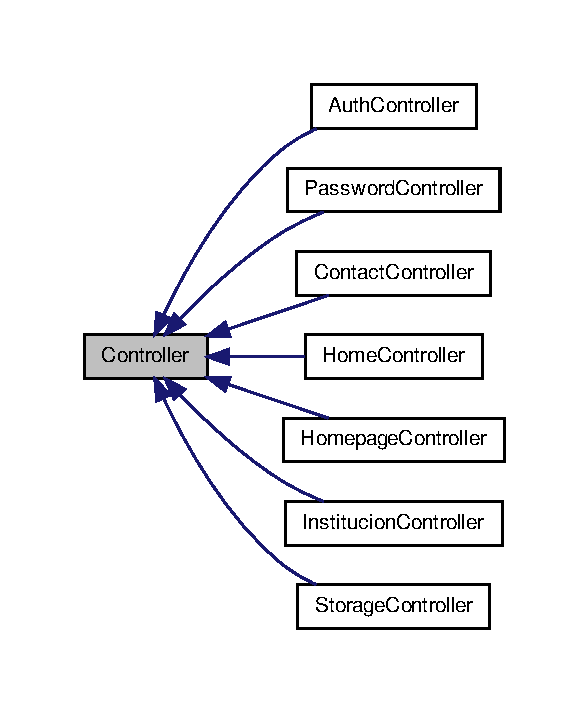
\includegraphics[width=282pt]{class_app_1_1_http_1_1_controllers_1_1_controller__inherit__graph}
\end{center}
\end{figure}
\subsection*{\-Métodos públicos}
\begin{DoxyCompactItemize}
\item 
\hypertarget{class_app_1_1_http_1_1_controllers_1_1_controller_a7acc2cc100af57a328fbc2e4469b9d6a}{{\bfseries listado\-\_\-instituciones} ()}\label{class_app_1_1_http_1_1_controllers_1_1_controller_a7acc2cc100af57a328fbc2e4469b9d6a}

\end{DoxyCompactItemize}


\-La documentación para esta clase fue generada a partir del siguiente fichero\-:\begin{DoxyCompactItemize}
\item 
/home/travis/build/tvargasvicencio/ayudalab/app/\-Http/\-Controllers/\-Controller.\-php\end{DoxyCompactItemize}

\hypertarget{class_crear_tabla_aviso}{\section{\-Referencia de la \-Clase \-Crear\-Tabla\-Aviso}
\label{class_crear_tabla_aviso}\index{\-Crear\-Tabla\-Aviso@{\-Crear\-Tabla\-Aviso}}
}
\subsection*{\-Métodos públicos}
\begin{DoxyCompactItemize}
\item 
\hyperlink{class_crear_tabla_aviso_a4edef5efd5ab94ce9d17295898ead93a}{up} ()
\item 
\hyperlink{class_crear_tabla_aviso_af5fda92f47a449c7a33f9dd5ef5aa6c3}{down} ()
\end{DoxyCompactItemize}


\subsection{\-Documentación de las funciones miembro}
\hypertarget{class_crear_tabla_aviso_af5fda92f47a449c7a33f9dd5ef5aa6c3}{\index{\-Crear\-Tabla\-Aviso@{\-Crear\-Tabla\-Aviso}!down@{down}}
\index{down@{down}!CrearTablaAviso@{\-Crear\-Tabla\-Aviso}}
\subsubsection[{down}]{\setlength{\rightskip}{0pt plus 5cm}{\bf down} (
\begin{DoxyParamCaption}
{}
\end{DoxyParamCaption}
)}}\label{class_crear_tabla_aviso_af5fda92f47a449c7a33f9dd5ef5aa6c3}
\-Reverse the migrations.

\begin{DoxyReturn}{\-Devuelve}
void 
\end{DoxyReturn}
\hypertarget{class_crear_tabla_aviso_a4edef5efd5ab94ce9d17295898ead93a}{\index{\-Crear\-Tabla\-Aviso@{\-Crear\-Tabla\-Aviso}!up@{up}}
\index{up@{up}!CrearTablaAviso@{\-Crear\-Tabla\-Aviso}}
\subsubsection[{up}]{\setlength{\rightskip}{0pt plus 5cm}{\bf up} (
\begin{DoxyParamCaption}
{}
\end{DoxyParamCaption}
)}}\label{class_crear_tabla_aviso_a4edef5efd5ab94ce9d17295898ead93a}
\-Run the migrations.

\begin{DoxyReturn}{\-Devuelve}
void 
\end{DoxyReturn}


\-La documentación para esta clase fue generada a partir del siguiente fichero\-:\begin{DoxyCompactItemize}
\item 
/home/travis/build/tvargasvicencio/ayudalab/database/migrations/2016\-\_\-11\-\_\-07\-\_\-194019\-\_\-crear\-\_\-tabla\-\_\-aviso.\-php\end{DoxyCompactItemize}

\hypertarget{class_crear_tabla_institucion}{\section{\-Referencia de la \-Clase \-Crear\-Tabla\-Institucion}
\label{class_crear_tabla_institucion}\index{\-Crear\-Tabla\-Institucion@{\-Crear\-Tabla\-Institucion}}
}
\subsection*{\-Métodos públicos}
\begin{DoxyCompactItemize}
\item 
\hyperlink{class_crear_tabla_institucion_a4edef5efd5ab94ce9d17295898ead93a}{up} ()
\item 
\hyperlink{class_crear_tabla_institucion_af5fda92f47a449c7a33f9dd5ef5aa6c3}{down} ()
\end{DoxyCompactItemize}


\subsection{\-Documentación de las funciones miembro}
\hypertarget{class_crear_tabla_institucion_af5fda92f47a449c7a33f9dd5ef5aa6c3}{\index{\-Crear\-Tabla\-Institucion@{\-Crear\-Tabla\-Institucion}!down@{down}}
\index{down@{down}!CrearTablaInstitucion@{\-Crear\-Tabla\-Institucion}}
\subsubsection[{down}]{\setlength{\rightskip}{0pt plus 5cm}{\bf down} (
\begin{DoxyParamCaption}
{}
\end{DoxyParamCaption}
)}}\label{class_crear_tabla_institucion_af5fda92f47a449c7a33f9dd5ef5aa6c3}
\-Reverse the migrations.

\begin{DoxyReturn}{\-Devuelve}
void 
\end{DoxyReturn}
\hypertarget{class_crear_tabla_institucion_a4edef5efd5ab94ce9d17295898ead93a}{\index{\-Crear\-Tabla\-Institucion@{\-Crear\-Tabla\-Institucion}!up@{up}}
\index{up@{up}!CrearTablaInstitucion@{\-Crear\-Tabla\-Institucion}}
\subsubsection[{up}]{\setlength{\rightskip}{0pt plus 5cm}{\bf up} (
\begin{DoxyParamCaption}
{}
\end{DoxyParamCaption}
)}}\label{class_crear_tabla_institucion_a4edef5efd5ab94ce9d17295898ead93a}
\-Run the migrations.

\begin{DoxyReturn}{\-Devuelve}
void 
\end{DoxyReturn}


\-La documentación para esta clase fue generada a partir del siguiente fichero\-:\begin{DoxyCompactItemize}
\item 
/home/travis/build/tvargasvicencio/ayudalab/database/migrations/2016\-\_\-11\-\_\-07\-\_\-192547\-\_\-crear\-\_\-tabla\-\_\-institucion.\-php\end{DoxyCompactItemize}

\hypertarget{class_create_password_resets_table}{\section{\-Referencia de la \-Clase \-Create\-Password\-Resets\-Table}
\label{class_create_password_resets_table}\index{\-Create\-Password\-Resets\-Table@{\-Create\-Password\-Resets\-Table}}
}
\subsection*{\-Métodos públicos}
\begin{DoxyCompactItemize}
\item 
\hyperlink{class_create_password_resets_table_a4edef5efd5ab94ce9d17295898ead93a}{up} ()
\item 
\hyperlink{class_create_password_resets_table_af5fda92f47a449c7a33f9dd5ef5aa6c3}{down} ()
\end{DoxyCompactItemize}


\subsection{\-Documentación de las funciones miembro}
\hypertarget{class_create_password_resets_table_af5fda92f47a449c7a33f9dd5ef5aa6c3}{\index{\-Create\-Password\-Resets\-Table@{\-Create\-Password\-Resets\-Table}!down@{down}}
\index{down@{down}!CreatePasswordResetsTable@{\-Create\-Password\-Resets\-Table}}
\subsubsection[{down}]{\setlength{\rightskip}{0pt plus 5cm}{\bf down} (
\begin{DoxyParamCaption}
{}
\end{DoxyParamCaption}
)}}\label{class_create_password_resets_table_af5fda92f47a449c7a33f9dd5ef5aa6c3}
\-Reverse the migrations.

\begin{DoxyReturn}{\-Devuelve}
void 
\end{DoxyReturn}
\hypertarget{class_create_password_resets_table_a4edef5efd5ab94ce9d17295898ead93a}{\index{\-Create\-Password\-Resets\-Table@{\-Create\-Password\-Resets\-Table}!up@{up}}
\index{up@{up}!CreatePasswordResetsTable@{\-Create\-Password\-Resets\-Table}}
\subsubsection[{up}]{\setlength{\rightskip}{0pt plus 5cm}{\bf up} (
\begin{DoxyParamCaption}
{}
\end{DoxyParamCaption}
)}}\label{class_create_password_resets_table_a4edef5efd5ab94ce9d17295898ead93a}
\-Run the migrations.

\begin{DoxyReturn}{\-Devuelve}
void 
\end{DoxyReturn}


\-La documentación para esta clase fue generada a partir del siguiente fichero\-:\begin{DoxyCompactItemize}
\item 
/home/travis/build/tvargasvicencio/ayudalab/database/migrations/2014\-\_\-10\-\_\-12\-\_\-100000\-\_\-create\-\_\-password\-\_\-resets\-\_\-table.\-php\end{DoxyCompactItemize}

\hypertarget{class_create_users_table}{\section{\-Referencia de la \-Clase \-Create\-Users\-Table}
\label{class_create_users_table}\index{\-Create\-Users\-Table@{\-Create\-Users\-Table}}
}
\subsection*{\-Métodos públicos}
\begin{DoxyCompactItemize}
\item 
\hyperlink{class_create_users_table_a4edef5efd5ab94ce9d17295898ead93a}{up} ()
\item 
\hyperlink{class_create_users_table_af5fda92f47a449c7a33f9dd5ef5aa6c3}{down} ()
\end{DoxyCompactItemize}


\subsection{\-Documentación de las funciones miembro}
\hypertarget{class_create_users_table_af5fda92f47a449c7a33f9dd5ef5aa6c3}{\index{\-Create\-Users\-Table@{\-Create\-Users\-Table}!down@{down}}
\index{down@{down}!CreateUsersTable@{\-Create\-Users\-Table}}
\subsubsection[{down}]{\setlength{\rightskip}{0pt plus 5cm}{\bf down} (
\begin{DoxyParamCaption}
{}
\end{DoxyParamCaption}
)}}\label{class_create_users_table_af5fda92f47a449c7a33f9dd5ef5aa6c3}
\-Reverse the migrations.

\begin{DoxyReturn}{\-Devuelve}
void 
\end{DoxyReturn}
\hypertarget{class_create_users_table_a4edef5efd5ab94ce9d17295898ead93a}{\index{\-Create\-Users\-Table@{\-Create\-Users\-Table}!up@{up}}
\index{up@{up}!CreateUsersTable@{\-Create\-Users\-Table}}
\subsubsection[{up}]{\setlength{\rightskip}{0pt plus 5cm}{\bf up} (
\begin{DoxyParamCaption}
{}
\end{DoxyParamCaption}
)}}\label{class_create_users_table_a4edef5efd5ab94ce9d17295898ead93a}
\-Run the migrations.

\begin{DoxyReturn}{\-Devuelve}
void 
\end{DoxyReturn}


\-La documentación para esta clase fue generada a partir del siguiente fichero\-:\begin{DoxyCompactItemize}
\item 
/home/travis/build/tvargasvicencio/ayudalab/database/migrations/2014\-\_\-10\-\_\-12\-\_\-000000\-\_\-create\-\_\-users\-\_\-table.\-php\end{DoxyCompactItemize}

\hypertarget{class_database_seeder}{\section{\-Referencia de la \-Clase \-Database\-Seeder}
\label{class_database_seeder}\index{\-Database\-Seeder@{\-Database\-Seeder}}
}
\subsection*{\-Métodos públicos}
\begin{DoxyCompactItemize}
\item 
\hyperlink{class_database_seeder_afb0fafe7e02a3ae1993c01c19fad2bae}{run} ()
\end{DoxyCompactItemize}


\subsection{\-Documentación de las funciones miembro}
\hypertarget{class_database_seeder_afb0fafe7e02a3ae1993c01c19fad2bae}{\index{\-Database\-Seeder@{\-Database\-Seeder}!run@{run}}
\index{run@{run}!DatabaseSeeder@{\-Database\-Seeder}}
\subsubsection[{run}]{\setlength{\rightskip}{0pt plus 5cm}{\bf run} (
\begin{DoxyParamCaption}
{}
\end{DoxyParamCaption}
)}}\label{class_database_seeder_afb0fafe7e02a3ae1993c01c19fad2bae}
\-Run the database seeds.

\begin{DoxyReturn}{\-Devuelve}
void 
\end{DoxyReturn}


\-La documentación para esta clase fue generada a partir del siguiente fichero\-:\begin{DoxyCompactItemize}
\item 
/home/travis/build/tvargasvicencio/ayudalab/database/seeds/\-Database\-Seeder.\-php\end{DoxyCompactItemize}

\hypertarget{class_example_test}{\section{\-Referencia de la \-Clase \-Example\-Test}
\label{class_example_test}\index{\-Example\-Test@{\-Example\-Test}}
}


\-Diagrama de herencias de \-Example\-Test
\nopagebreak
\begin{figure}[H]
\begin{center}
\leavevmode
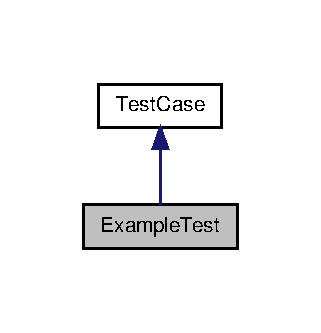
\includegraphics[width=154pt]{class_example_test__inherit__graph}
\end{center}
\end{figure}


\-Diagrama de colaboración para \-Example\-Test\-:
\nopagebreak
\begin{figure}[H]
\begin{center}
\leavevmode
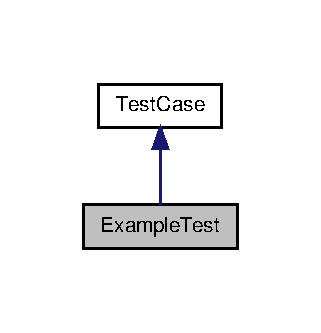
\includegraphics[width=154pt]{class_example_test__coll__graph}
\end{center}
\end{figure}
\subsection*{\-Métodos públicos}
\begin{DoxyCompactItemize}
\item 
\hyperlink{class_example_test_a2e9e13cc943cabece2a00a67d36abc0e}{test\-Basic\-Example} ()
\end{DoxyCompactItemize}


\subsection{\-Documentación de las funciones miembro}
\hypertarget{class_example_test_a2e9e13cc943cabece2a00a67d36abc0e}{\index{\-Example\-Test@{\-Example\-Test}!test\-Basic\-Example@{test\-Basic\-Example}}
\index{test\-Basic\-Example@{test\-Basic\-Example}!ExampleTest@{\-Example\-Test}}
\subsubsection[{test\-Basic\-Example}]{\setlength{\rightskip}{0pt plus 5cm}{\bf test\-Basic\-Example} (
\begin{DoxyParamCaption}
{}
\end{DoxyParamCaption}
)}}\label{class_example_test_a2e9e13cc943cabece2a00a67d36abc0e}
\-A basic functional test example.

\begin{DoxyReturn}{\-Devuelve}
void 
\end{DoxyReturn}


\-La documentación para esta clase fue generada a partir del siguiente fichero\-:\begin{DoxyCompactItemize}
\item 
/home/travis/build/tvargasvicencio/ayudalab/tests/\-Example\-Test.\-php\end{DoxyCompactItemize}

\hypertarget{class_app_1_1_http_1_1_controllers_1_1_home_controller}{\section{\-Referencia de la \-Clase \-Home\-Controller}
\label{class_app_1_1_http_1_1_controllers_1_1_home_controller}\index{\-Home\-Controller@{\-Home\-Controller}}
}


\-Diagrama de herencias de \-Home\-Controller
\nopagebreak
\begin{figure}[H]
\begin{center}
\leavevmode
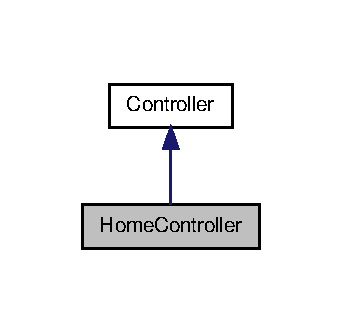
\includegraphics[width=164pt]{class_app_1_1_http_1_1_controllers_1_1_home_controller__inherit__graph}
\end{center}
\end{figure}


\-Diagrama de colaboración para \-Home\-Controller\-:
\nopagebreak
\begin{figure}[H]
\begin{center}
\leavevmode
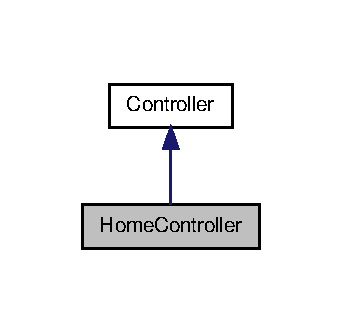
\includegraphics[width=164pt]{class_app_1_1_http_1_1_controllers_1_1_home_controller__coll__graph}
\end{center}
\end{figure}
\subsection*{\-Métodos públicos}
\begin{DoxyCompactItemize}
\item 
\hyperlink{class_app_1_1_http_1_1_controllers_1_1_home_controller_a095c5d389db211932136b53f25f39685}{\-\_\-\-\_\-construct} ()
\item 
\hyperlink{class_app_1_1_http_1_1_controllers_1_1_home_controller_a149eb92716c1084a935e04a8d95f7347}{index} ()
\item 
\hyperlink{class_app_1_1_http_1_1_controllers_1_1_home_controller_a2b9266e19e6e9224aaae7b4c7836ff40}{informacion\-Institucional} ()
\item 
\hyperlink{class_app_1_1_http_1_1_controllers_1_1_home_controller_adb42f8dc18c16f7d581c3615a03d6f75}{editar\-Informacion\-Institucional} (\-Request \$request)
\item 
\hyperlink{class_app_1_1_http_1_1_controllers_1_1_home_controller_ad1992463a8d72baca9db54556e0ada5a}{nuevo\-Aviso} ()
\item 
\hyperlink{class_app_1_1_http_1_1_controllers_1_1_home_controller_aa8267c0b6eb2bb4b99276eee892b81cd}{guardar\-Nuevo\-Aviso} (\-Request \$request)
\item 
\hyperlink{class_app_1_1_http_1_1_controllers_1_1_home_controller_a599f5b2f09e9ab0cba15ac2e08e2d3a4}{lista\-Avisos} ()
\item 
\hyperlink{class_app_1_1_http_1_1_controllers_1_1_home_controller_a75d08b7be79fbf0f19475105c86543fc}{eliminar\-Aviso} (\-Request \$request)
\item 
\hyperlink{class_app_1_1_http_1_1_controllers_1_1_home_controller_a38e591dabfd118030440ef4c003cc08f}{editar\-Aviso} (\$institucion, \$aviso)
\item 
\hyperlink{class_app_1_1_http_1_1_controllers_1_1_home_controller_a7a9cc6d3be72174f7e315185572208ac}{guardar\-Editar\-Aviso} (\-Request \$request)
\item 
\hyperlink{class_app_1_1_http_1_1_controllers_1_1_home_controller_a2c26c9b748066e4f390ee5172daa72b2}{estadisticas} ()
\end{DoxyCompactItemize}


\subsection{\-Documentación del constructor y destructor}
\hypertarget{class_app_1_1_http_1_1_controllers_1_1_home_controller_a095c5d389db211932136b53f25f39685}{\index{\-App\-::\-Http\-::\-Controllers\-::\-Home\-Controller@{\-App\-::\-Http\-::\-Controllers\-::\-Home\-Controller}!\-\_\-\-\_\-construct@{\-\_\-\-\_\-construct}}
\index{\-\_\-\-\_\-construct@{\-\_\-\-\_\-construct}!App::Http::Controllers::HomeController@{\-App\-::\-Http\-::\-Controllers\-::\-Home\-Controller}}
\subsubsection[{\-\_\-\-\_\-construct}]{\setlength{\rightskip}{0pt plus 5cm}{\bf \-\_\-\-\_\-construct} (
\begin{DoxyParamCaption}
{}
\end{DoxyParamCaption}
)}}\label{class_app_1_1_http_1_1_controllers_1_1_home_controller_a095c5d389db211932136b53f25f39685}
\-Middleware para otorgar acceso solo a un usuario autenticado 

\subsection{\-Documentación de las funciones miembro}
\hypertarget{class_app_1_1_http_1_1_controllers_1_1_home_controller_a38e591dabfd118030440ef4c003cc08f}{\index{\-App\-::\-Http\-::\-Controllers\-::\-Home\-Controller@{\-App\-::\-Http\-::\-Controllers\-::\-Home\-Controller}!editar\-Aviso@{editar\-Aviso}}
\index{editar\-Aviso@{editar\-Aviso}!App::Http::Controllers::HomeController@{\-App\-::\-Http\-::\-Controllers\-::\-Home\-Controller}}
\subsubsection[{editar\-Aviso}]{\setlength{\rightskip}{0pt plus 5cm}{\bf editar\-Aviso} (
\begin{DoxyParamCaption}
\item[{\$}]{institucion, }
\item[{\$}]{aviso}
\end{DoxyParamCaption}
)}}\label{class_app_1_1_http_1_1_controllers_1_1_home_controller_a38e591dabfd118030440ef4c003cc08f}
\-Recibe petición \-G\-E\-T a 'dashboard/institucion/\{institucion?\}/aviso/\{aviso?\}' \-Retorna la vista con el formulario para editar el aviso


\begin{DoxyParams}{\-Parámetros}
{\em $<$type$>$} & \$institucion \-El nombre de la institución dueña del aviso \\
\hline
{\em $<$type$>$} & \$aviso \-E\-L \-I\-D del aviso\\
\hline
\end{DoxyParams}
\begin{DoxyReturn}{\-Devuelve}
$<$type$>$ ( description\-\_\-of\-\_\-the\-\_\-return\-\_\-value ) 
\end{DoxyReturn}
\hypertarget{class_app_1_1_http_1_1_controllers_1_1_home_controller_adb42f8dc18c16f7d581c3615a03d6f75}{\index{\-App\-::\-Http\-::\-Controllers\-::\-Home\-Controller@{\-App\-::\-Http\-::\-Controllers\-::\-Home\-Controller}!editar\-Informacion\-Institucional@{editar\-Informacion\-Institucional}}
\index{editar\-Informacion\-Institucional@{editar\-Informacion\-Institucional}!App::Http::Controllers::HomeController@{\-App\-::\-Http\-::\-Controllers\-::\-Home\-Controller}}
\subsubsection[{editar\-Informacion\-Institucional}]{\setlength{\rightskip}{0pt plus 5cm}{\bf editar\-Informacion\-Institucional} (
\begin{DoxyParamCaption}
\item[{\-Request \$}]{request}
\end{DoxyParamCaption}
)}}\label{class_app_1_1_http_1_1_controllers_1_1_home_controller_adb42f8dc18c16f7d581c3615a03d6f75}
\-Recibe petición \-P\-O\-S\-T a '/dashboard/informacion\-Institucional' \-Recibe formulario vía \-A\-J\-A\-X y lo valida con \-Validator \-Si encuentra errores, devuelve una lista de errores para mostrarlos en la vista \-Sino, obtiene la institución y actualiza los datos


\begin{DoxyParams}{\-Parámetros}
{\em $\backslash$\-Illuminate$\backslash$\-Http$\backslash$\-Request} & \$request \-The request\\
\hline
\end{DoxyParams}
\begin{DoxyReturn}{\-Devuelve}
$<$type$>$ ( description\-\_\-of\-\_\-the\-\_\-return\-\_\-value ) 
\end{DoxyReturn}
\hypertarget{class_app_1_1_http_1_1_controllers_1_1_home_controller_a75d08b7be79fbf0f19475105c86543fc}{\index{\-App\-::\-Http\-::\-Controllers\-::\-Home\-Controller@{\-App\-::\-Http\-::\-Controllers\-::\-Home\-Controller}!eliminar\-Aviso@{eliminar\-Aviso}}
\index{eliminar\-Aviso@{eliminar\-Aviso}!App::Http::Controllers::HomeController@{\-App\-::\-Http\-::\-Controllers\-::\-Home\-Controller}}
\subsubsection[{eliminar\-Aviso}]{\setlength{\rightskip}{0pt plus 5cm}{\bf eliminar\-Aviso} (
\begin{DoxyParamCaption}
\item[{\-Request \$}]{request}
\end{DoxyParamCaption}
)}}\label{class_app_1_1_http_1_1_controllers_1_1_home_controller_a75d08b7be79fbf0f19475105c86543fc}
\-Recibe petición \-P\-O\-S\-T a '/dashboard/lista\-Avisos/eliminar\-Aviso' \-Recibe la 'id' del aviso vía \-A\-J\-A\-X \-Verifica que el aviso corresponda a un aviso del usuario logueado y lo borra


\begin{DoxyParams}{\-Parámetros}
{\em $\backslash$\-Illuminate$\backslash$\-Http$\backslash$\-Request} & \$request \-The request\\
\hline
\end{DoxyParams}
\begin{DoxyReturn}{\-Devuelve}
$<$type$>$ ( description\-\_\-of\-\_\-the\-\_\-return\-\_\-value ) 
\end{DoxyReturn}
\hypertarget{class_app_1_1_http_1_1_controllers_1_1_home_controller_a2c26c9b748066e4f390ee5172daa72b2}{\index{\-App\-::\-Http\-::\-Controllers\-::\-Home\-Controller@{\-App\-::\-Http\-::\-Controllers\-::\-Home\-Controller}!estadisticas@{estadisticas}}
\index{estadisticas@{estadisticas}!App::Http::Controllers::HomeController@{\-App\-::\-Http\-::\-Controllers\-::\-Home\-Controller}}
\subsubsection[{estadisticas}]{\setlength{\rightskip}{0pt plus 5cm}{\bf estadisticas} (
\begin{DoxyParamCaption}
{}
\end{DoxyParamCaption}
)}}\label{class_app_1_1_http_1_1_controllers_1_1_home_controller_a2c26c9b748066e4f390ee5172daa72b2}
\-Recibe petición \-G\-E\-T a '/dashboard/estadisticas' \-Retorna la vista con estadísticas falsas (por ahora)

\begin{DoxyReturn}{\-Devuelve}
$<$type$>$ ( description\-\_\-of\-\_\-the\-\_\-return\-\_\-value ) 
\end{DoxyReturn}
\hypertarget{class_app_1_1_http_1_1_controllers_1_1_home_controller_a7a9cc6d3be72174f7e315185572208ac}{\index{\-App\-::\-Http\-::\-Controllers\-::\-Home\-Controller@{\-App\-::\-Http\-::\-Controllers\-::\-Home\-Controller}!guardar\-Editar\-Aviso@{guardar\-Editar\-Aviso}}
\index{guardar\-Editar\-Aviso@{guardar\-Editar\-Aviso}!App::Http::Controllers::HomeController@{\-App\-::\-Http\-::\-Controllers\-::\-Home\-Controller}}
\subsubsection[{guardar\-Editar\-Aviso}]{\setlength{\rightskip}{0pt plus 5cm}{\bf guardar\-Editar\-Aviso} (
\begin{DoxyParamCaption}
\item[{\-Request \$}]{request}
\end{DoxyParamCaption}
)}}\label{class_app_1_1_http_1_1_controllers_1_1_home_controller_a7a9cc6d3be72174f7e315185572208ac}
\-Recibe petición \-P\-O\-S\-T a 'dashboard/institucion/\{institucion?\}/aviso/\{aviso?\}' \-Recibe formulario vía \-A\-J\-A\-X y lo valida con \-Validator \-Si encuentra errores, devuelve una lista de errores para mostrarlos en la vista \-Sino, busca el aviso y verifica que corresponda al usuario logueado \-Guarda el aviso modificado


\begin{DoxyParams}{\-Parámetros}
{\em $\backslash$\-Illuminate$\backslash$\-Http$\backslash$\-Request} & \$request \-The request\\
\hline
\end{DoxyParams}
\begin{DoxyReturn}{\-Devuelve}
$<$type$>$ ( description\-\_\-of\-\_\-the\-\_\-return\-\_\-value ) 
\end{DoxyReturn}
\hypertarget{class_app_1_1_http_1_1_controllers_1_1_home_controller_aa8267c0b6eb2bb4b99276eee892b81cd}{\index{\-App\-::\-Http\-::\-Controllers\-::\-Home\-Controller@{\-App\-::\-Http\-::\-Controllers\-::\-Home\-Controller}!guardar\-Nuevo\-Aviso@{guardar\-Nuevo\-Aviso}}
\index{guardar\-Nuevo\-Aviso@{guardar\-Nuevo\-Aviso}!App::Http::Controllers::HomeController@{\-App\-::\-Http\-::\-Controllers\-::\-Home\-Controller}}
\subsubsection[{guardar\-Nuevo\-Aviso}]{\setlength{\rightskip}{0pt plus 5cm}{\bf guardar\-Nuevo\-Aviso} (
\begin{DoxyParamCaption}
\item[{\-Request \$}]{request}
\end{DoxyParamCaption}
)}}\label{class_app_1_1_http_1_1_controllers_1_1_home_controller_aa8267c0b6eb2bb4b99276eee892b81cd}
\-Recibe petición \-P\-O\-S\-T a '/dashboard/nuevo\-Aviso' \-Recibe formulario vía \-A\-J\-A\-X y lo valida con \-Validator \-Si encuentra errores, devuelve una lista de errores para mostrarlos en la vista \-Sino, crea el nuevo aviso y lo guarda en \-B\-D


\begin{DoxyParams}{\-Parámetros}
{\em $\backslash$\-Illuminate$\backslash$\-Http$\backslash$\-Request} & \$request \-The request\\
\hline
\end{DoxyParams}
\begin{DoxyReturn}{\-Devuelve}
$<$type$>$ ( description\-\_\-of\-\_\-the\-\_\-return\-\_\-value ) 
\end{DoxyReturn}
\hypertarget{class_app_1_1_http_1_1_controllers_1_1_home_controller_a149eb92716c1084a935e04a8d95f7347}{\index{\-App\-::\-Http\-::\-Controllers\-::\-Home\-Controller@{\-App\-::\-Http\-::\-Controllers\-::\-Home\-Controller}!index@{index}}
\index{index@{index}!App::Http::Controllers::HomeController@{\-App\-::\-Http\-::\-Controllers\-::\-Home\-Controller}}
\subsubsection[{index}]{\setlength{\rightskip}{0pt plus 5cm}{\bf index} (
\begin{DoxyParamCaption}
{}
\end{DoxyParamCaption}
)}}\label{class_app_1_1_http_1_1_controllers_1_1_home_controller_a149eb92716c1084a935e04a8d95f7347}
\-Revisa si el usuario actual está autenticado \-Devuelve un objeto con el usuario logueado y otro de su institución correspondiente

\begin{DoxyReturn}{\-Devuelve}
$<$type$>$ ( description\-\_\-of\-\_\-the\-\_\-return\-\_\-value ) 
\end{DoxyReturn}
\hypertarget{class_app_1_1_http_1_1_controllers_1_1_home_controller_a2b9266e19e6e9224aaae7b4c7836ff40}{\index{\-App\-::\-Http\-::\-Controllers\-::\-Home\-Controller@{\-App\-::\-Http\-::\-Controllers\-::\-Home\-Controller}!informacion\-Institucional@{informacion\-Institucional}}
\index{informacion\-Institucional@{informacion\-Institucional}!App::Http::Controllers::HomeController@{\-App\-::\-Http\-::\-Controllers\-::\-Home\-Controller}}
\subsubsection[{informacion\-Institucional}]{\setlength{\rightskip}{0pt plus 5cm}{\bf informacion\-Institucional} (
\begin{DoxyParamCaption}
{}
\end{DoxyParamCaption}
)}}\label{class_app_1_1_http_1_1_controllers_1_1_home_controller_a2b9266e19e6e9224aaae7b4c7836ff40}
\-Recibe petición \-G\-E\-T a '/dashboard/informacion\-Institucional' \-Retorna la vista para editar la información institucional en el dashboard

\begin{DoxyReturn}{\-Devuelve}
$<$type$>$ ( description\-\_\-of\-\_\-the\-\_\-return\-\_\-value ) 
\end{DoxyReturn}
\hypertarget{class_app_1_1_http_1_1_controllers_1_1_home_controller_a599f5b2f09e9ab0cba15ac2e08e2d3a4}{\index{\-App\-::\-Http\-::\-Controllers\-::\-Home\-Controller@{\-App\-::\-Http\-::\-Controllers\-::\-Home\-Controller}!lista\-Avisos@{lista\-Avisos}}
\index{lista\-Avisos@{lista\-Avisos}!App::Http::Controllers::HomeController@{\-App\-::\-Http\-::\-Controllers\-::\-Home\-Controller}}
\subsubsection[{lista\-Avisos}]{\setlength{\rightskip}{0pt plus 5cm}{\bf lista\-Avisos} (
\begin{DoxyParamCaption}
{}
\end{DoxyParamCaption}
)}}\label{class_app_1_1_http_1_1_controllers_1_1_home_controller_a599f5b2f09e9ab0cba15ac2e08e2d3a4}
\-Recibe petición \-G\-E\-T a '/dashboard/lista\-Avisos' \-Retorna la vista con los avisos de la institución, ordenados según más reciente de a 6 por página

\begin{DoxyReturn}{\-Devuelve}
$<$type$>$ ( description\-\_\-of\-\_\-the\-\_\-return\-\_\-value ) 
\end{DoxyReturn}
\hypertarget{class_app_1_1_http_1_1_controllers_1_1_home_controller_ad1992463a8d72baca9db54556e0ada5a}{\index{\-App\-::\-Http\-::\-Controllers\-::\-Home\-Controller@{\-App\-::\-Http\-::\-Controllers\-::\-Home\-Controller}!nuevo\-Aviso@{nuevo\-Aviso}}
\index{nuevo\-Aviso@{nuevo\-Aviso}!App::Http::Controllers::HomeController@{\-App\-::\-Http\-::\-Controllers\-::\-Home\-Controller}}
\subsubsection[{nuevo\-Aviso}]{\setlength{\rightskip}{0pt plus 5cm}{\bf nuevo\-Aviso} (
\begin{DoxyParamCaption}
{}
\end{DoxyParamCaption}
)}}\label{class_app_1_1_http_1_1_controllers_1_1_home_controller_ad1992463a8d72baca9db54556e0ada5a}
\-Recibe petición \-G\-E\-T a '/dashboard/nuevo\-Aviso' \-Retorna la vista con el formulario para crear un nuevo aviso

\begin{DoxyReturn}{\-Devuelve}
$<$type$>$ ( description\-\_\-of\-\_\-the\-\_\-return\-\_\-value ) 
\end{DoxyReturn}


\-La documentación para esta clase fue generada a partir del siguiente fichero\-:\begin{DoxyCompactItemize}
\item 
/home/travis/build/tvargasvicencio/ayudalab/app/\-Http/\-Controllers/\-Home\-Controller.\-php\end{DoxyCompactItemize}

\hypertarget{class_app_1_1_http_1_1_controllers_1_1_homepage_controller}{\section{\-Referencia de la \-Clase \-Homepage\-Controller}
\label{class_app_1_1_http_1_1_controllers_1_1_homepage_controller}\index{\-Homepage\-Controller@{\-Homepage\-Controller}}
}


\-Diagrama de herencias de \-Homepage\-Controller
\nopagebreak
\begin{figure}[H]
\begin{center}
\leavevmode
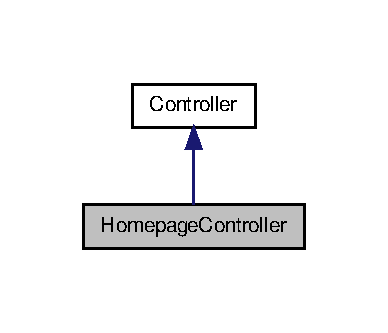
\includegraphics[width=186pt]{class_app_1_1_http_1_1_controllers_1_1_homepage_controller__inherit__graph}
\end{center}
\end{figure}


\-Diagrama de colaboración para \-Homepage\-Controller\-:
\nopagebreak
\begin{figure}[H]
\begin{center}
\leavevmode
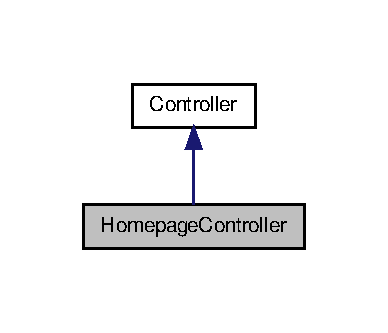
\includegraphics[width=186pt]{class_app_1_1_http_1_1_controllers_1_1_homepage_controller__coll__graph}
\end{center}
\end{figure}
\subsection*{\-Métodos públicos}
\begin{DoxyCompactItemize}
\item 
\hyperlink{class_app_1_1_http_1_1_controllers_1_1_homepage_controller_a149eb92716c1084a935e04a8d95f7347}{index} ()
\end{DoxyCompactItemize}


\subsection{\-Documentación de las funciones miembro}
\hypertarget{class_app_1_1_http_1_1_controllers_1_1_homepage_controller_a149eb92716c1084a935e04a8d95f7347}{\index{\-App\-::\-Http\-::\-Controllers\-::\-Homepage\-Controller@{\-App\-::\-Http\-::\-Controllers\-::\-Homepage\-Controller}!index@{index}}
\index{index@{index}!App::Http::Controllers::HomepageController@{\-App\-::\-Http\-::\-Controllers\-::\-Homepage\-Controller}}
\subsubsection[{index}]{\setlength{\rightskip}{0pt plus 5cm}{\bf index} (
\begin{DoxyParamCaption}
{}
\end{DoxyParamCaption}
)}}\label{class_app_1_1_http_1_1_controllers_1_1_homepage_controller_a149eb92716c1084a935e04a8d95f7347}
\-Recibe petición \-G\-E\-T a '/' \-Retorna la paǵina principal de \-Socialbook

\begin{DoxyReturn}{\-Devuelve}
$<$type$>$ ( description\-\_\-of\-\_\-the\-\_\-return\-\_\-value ) 
\end{DoxyReturn}


\-La documentación para esta clase fue generada a partir del siguiente fichero\-:\begin{DoxyCompactItemize}
\item 
/home/travis/build/tvargasvicencio/ayudalab/app/\-Http/\-Controllers/\-Homepage\-Controller.\-php\end{DoxyCompactItemize}

\hypertarget{class_app_1_1_imagen}{\section{\-Referencia de la \-Clase \-Imagen}
\label{class_app_1_1_imagen}\index{\-Imagen@{\-Imagen}}
}
\subsection*{\-Métodos públicos}
\begin{DoxyCompactItemize}
\item 
\hypertarget{class_app_1_1_imagen_abfb0e179daf0a8f710adbb1456e5b3eb}{{\bfseries institucion} ()}\label{class_app_1_1_imagen_abfb0e179daf0a8f710adbb1456e5b3eb}

\end{DoxyCompactItemize}
\subsection*{\-Atributos protegidos}
\begin{DoxyCompactItemize}
\item 
\hypertarget{class_app_1_1_imagen_aab581066837d6296ba35c72937b6fc1c}{{\bfseries \$dates} = \mbox{[}'deleted\-\_\-at'\mbox{]}}\label{class_app_1_1_imagen_aab581066837d6296ba35c72937b6fc1c}

\item 
\hypertarget{class_app_1_1_imagen_ae8876a14058f368335baccf35af4a22b}{{\bfseries \$table} = 'imagen\-\_\-institucion'}\label{class_app_1_1_imagen_ae8876a14058f368335baccf35af4a22b}

\item 
\hypertarget{class_app_1_1_imagen_a5758640ec23bdc1a6850649763244e86}{{\bfseries \$guarded} = \mbox{[}$\,$\mbox{]}}\label{class_app_1_1_imagen_a5758640ec23bdc1a6850649763244e86}

\item 
\hypertarget{class_app_1_1_imagen_a927b0256b942a3ee89485f2649af7981}{{\bfseries \$primary\-Key} = 'id\-\_\-imagen'}\label{class_app_1_1_imagen_a927b0256b942a3ee89485f2649af7981}

\end{DoxyCompactItemize}


\-La documentación para esta clase fue generada a partir del siguiente fichero\-:\begin{DoxyCompactItemize}
\item 
/home/travis/build/tvargasvicencio/ayudalab/app/\-Imagen.\-php\end{DoxyCompactItemize}

\hypertarget{class_imagen_aviso}{\section{\-Referencia de la \-Clase \-Imagen\-Aviso}
\label{class_imagen_aviso}\index{\-Imagen\-Aviso@{\-Imagen\-Aviso}}
}
\subsection*{\-Métodos públicos}
\begin{DoxyCompactItemize}
\item 
\hyperlink{class_imagen_aviso_afb0fafe7e02a3ae1993c01c19fad2bae}{run} ()
\end{DoxyCompactItemize}


\subsection{\-Documentación de las funciones miembro}
\hypertarget{class_imagen_aviso_afb0fafe7e02a3ae1993c01c19fad2bae}{\index{\-Imagen\-Aviso@{\-Imagen\-Aviso}!run@{run}}
\index{run@{run}!ImagenAviso@{\-Imagen\-Aviso}}
\subsubsection[{run}]{\setlength{\rightskip}{0pt plus 5cm}{\bf run} (
\begin{DoxyParamCaption}
{}
\end{DoxyParamCaption}
)}}\label{class_imagen_aviso_afb0fafe7e02a3ae1993c01c19fad2bae}
\-Run the database seeds.

\begin{DoxyReturn}{\-Devuelve}
void 
\end{DoxyReturn}


\-La documentación para esta clase fue generada a partir del siguiente fichero\-:\begin{DoxyCompactItemize}
\item 
/home/travis/build/tvargasvicencio/ayudalab/database/seeds/\-Imagen\-Aviso.\-php\end{DoxyCompactItemize}

\hypertarget{class_app_1_1_imagen_evento}{\section{\-Referencia de la \-Clase \-Imagen\-Evento}
\label{class_app_1_1_imagen_evento}\index{\-Imagen\-Evento@{\-Imagen\-Evento}}
}
\subsection*{\-Métodos públicos}
\begin{DoxyCompactItemize}
\item 
\hypertarget{class_app_1_1_imagen_evento_a893f830558ee917f86dae4c21bc95319}{{\bfseries aviso} ()}\label{class_app_1_1_imagen_evento_a893f830558ee917f86dae4c21bc95319}

\item 
\hypertarget{class_app_1_1_imagen_evento_aa200b538a8030385bdf5c02a9f2216ad}{{\bfseries noticia} ()}\label{class_app_1_1_imagen_evento_aa200b538a8030385bdf5c02a9f2216ad}

\end{DoxyCompactItemize}
\subsection*{\-Atributos protegidos}
\begin{DoxyCompactItemize}
\item 
\hypertarget{class_app_1_1_imagen_evento_aab581066837d6296ba35c72937b6fc1c}{{\bfseries \$dates} = \mbox{[}'deleted\-\_\-at'\mbox{]}}\label{class_app_1_1_imagen_evento_aab581066837d6296ba35c72937b6fc1c}

\item 
\hypertarget{class_app_1_1_imagen_evento_ae8876a14058f368335baccf35af4a22b}{{\bfseries \$table} = 'imagen\-\_\-evento'}\label{class_app_1_1_imagen_evento_ae8876a14058f368335baccf35af4a22b}

\item 
\hypertarget{class_app_1_1_imagen_evento_a5758640ec23bdc1a6850649763244e86}{{\bfseries \$guarded} = \mbox{[}$\,$\mbox{]}}\label{class_app_1_1_imagen_evento_a5758640ec23bdc1a6850649763244e86}

\item 
\hypertarget{class_app_1_1_imagen_evento_a927b0256b942a3ee89485f2649af7981}{{\bfseries \$primary\-Key} = 'id\-\_\-imagen'}\label{class_app_1_1_imagen_evento_a927b0256b942a3ee89485f2649af7981}

\end{DoxyCompactItemize}


\-La documentación para esta clase fue generada a partir del siguiente fichero\-:\begin{DoxyCompactItemize}
\item 
/home/travis/build/tvargasvicencio/ayudalab/app/\-Imagen\-Evento.\-php\end{DoxyCompactItemize}

\hypertarget{class_imagen_table_seeder}{\section{\-Referencia de la \-Clase \-Imagen\-Table\-Seeder}
\label{class_imagen_table_seeder}\index{\-Imagen\-Table\-Seeder@{\-Imagen\-Table\-Seeder}}
}
\subsection*{\-Métodos públicos}
\begin{DoxyCompactItemize}
\item 
\hyperlink{class_imagen_table_seeder_afb0fafe7e02a3ae1993c01c19fad2bae}{run} ()
\end{DoxyCompactItemize}


\subsection{\-Documentación de las funciones miembro}
\hypertarget{class_imagen_table_seeder_afb0fafe7e02a3ae1993c01c19fad2bae}{\index{\-Imagen\-Table\-Seeder@{\-Imagen\-Table\-Seeder}!run@{run}}
\index{run@{run}!ImagenTableSeeder@{\-Imagen\-Table\-Seeder}}
\subsubsection[{run}]{\setlength{\rightskip}{0pt plus 5cm}{\bf run} (
\begin{DoxyParamCaption}
{}
\end{DoxyParamCaption}
)}}\label{class_imagen_table_seeder_afb0fafe7e02a3ae1993c01c19fad2bae}
\-Run the database seeds.

\begin{DoxyReturn}{\-Devuelve}
void 
\end{DoxyReturn}


\-La documentación para esta clase fue generada a partir del siguiente fichero\-:\begin{DoxyCompactItemize}
\item 
/home/travis/build/tvargasvicencio/ayudalab/database/seeds/\-Imagen\-Table\-Seeder.\-php\end{DoxyCompactItemize}

\hypertarget{class_app_1_1_institucion}{\section{\-Referencia de la \-Clase \-Institucion}
\label{class_app_1_1_institucion}\index{\-Institucion@{\-Institucion}}
}
\subsection*{\-Métodos públicos}
\begin{DoxyCompactItemize}
\item 
\hyperlink{class_app_1_1_institucion_ade152cc7eb49d82f41821a9219c4268f}{avisos} ()
\item 
\hypertarget{class_app_1_1_institucion_a839cc211520cee7e68f28fe9c6f08a56}{{\bfseries noticias} ()}\label{class_app_1_1_institucion_a839cc211520cee7e68f28fe9c6f08a56}

\item 
\hypertarget{class_app_1_1_institucion_a5dc675056de3625bba3841341313ff72}{{\bfseries imagen} ()}\label{class_app_1_1_institucion_a5dc675056de3625bba3841341313ff72}

\item 
\hyperlink{class_app_1_1_institucion_ae8a275690ff1b618e1947378b0ed73ae}{user} ()
\end{DoxyCompactItemize}
\subsection*{\-Atributos protegidos}
\begin{DoxyCompactItemize}
\item 
\hypertarget{class_app_1_1_institucion_aab581066837d6296ba35c72937b6fc1c}{{\bfseries \$dates} = \mbox{[}'deleted\-\_\-at'\mbox{]}}\label{class_app_1_1_institucion_aab581066837d6296ba35c72937b6fc1c}

\item 
\hypertarget{class_app_1_1_institucion_ae8876a14058f368335baccf35af4a22b}{{\bfseries \$table} = 'institucion'}\label{class_app_1_1_institucion_ae8876a14058f368335baccf35af4a22b}

\item 
\hypertarget{class_app_1_1_institucion_a927b0256b942a3ee89485f2649af7981}{{\bfseries \$primary\-Key} = \char`\"{}id\-\_\-institucion\char`\"{}}\label{class_app_1_1_institucion_a927b0256b942a3ee89485f2649af7981}

\item 
{\bfseries \$fillable}
\end{DoxyCompactItemize}


\subsection{\-Documentación de las funciones miembro}
\hypertarget{class_app_1_1_institucion_ade152cc7eb49d82f41821a9219c4268f}{\index{\-App\-::\-Institucion@{\-App\-::\-Institucion}!avisos@{avisos}}
\index{avisos@{avisos}!App::Institucion@{\-App\-::\-Institucion}}
\subsubsection[{avisos}]{\setlength{\rightskip}{0pt plus 5cm}{\bf avisos} (
\begin{DoxyParamCaption}
{}
\end{DoxyParamCaption}
)}}\label{class_app_1_1_institucion_ade152cc7eb49d82f41821a9219c4268f}
\-Indica que una \-Institución puede tener muchos aviso

\begin{DoxyReturn}{\-Devuelve}
$<$type$>$ ( description\-\_\-of\-\_\-the\-\_\-return\-\_\-value ) 
\end{DoxyReturn}
\hypertarget{class_app_1_1_institucion_ae8a275690ff1b618e1947378b0ed73ae}{\index{\-App\-::\-Institucion@{\-App\-::\-Institucion}!user@{user}}
\index{user@{user}!App::Institucion@{\-App\-::\-Institucion}}
\subsubsection[{user}]{\setlength{\rightskip}{0pt plus 5cm}{\bf user} (
\begin{DoxyParamCaption}
{}
\end{DoxyParamCaption}
)}}\label{class_app_1_1_institucion_ae8a275690ff1b618e1947378b0ed73ae}
\-Indica que una \-Institución puede tener muchos user

\begin{DoxyReturn}{\-Devuelve}
$<$type$>$ ( description\-\_\-of\-\_\-the\-\_\-return\-\_\-value ) 
\end{DoxyReturn}


\subsection{\-Documentación de los campos}
\hypertarget{class_app_1_1_institucion_a6a90e74ccdf5efd70d51d10c906f8e32}{\index{\-App\-::\-Institucion@{\-App\-::\-Institucion}!\$fillable@{\$fillable}}
\index{\$fillable@{\$fillable}!App::Institucion@{\-App\-::\-Institucion}}
\subsubsection[{\$fillable}]{\setlength{\rightskip}{0pt plus 5cm}\$fillable\hspace{0.3cm}{\ttfamily  \mbox{[}protected\mbox{]}}}}\label{class_app_1_1_institucion_a6a90e74ccdf5efd70d51d10c906f8e32}
{\bfseries \-Valor inicial\-:}
\begin{DoxyCode}
 ['rut_inst',
        'mision',
        'vision',
        'nombre',
        'direccion',
        'telefono',
        'mail']
\end{DoxyCode}


\-La documentación para esta clase fue generada a partir del siguiente fichero\-:\begin{DoxyCompactItemize}
\item 
/home/travis/build/tvargasvicencio/ayudalab/app/\-Institucion.\-php\end{DoxyCompactItemize}

\hypertarget{class_app_1_1_http_1_1_controllers_1_1_institucion_controller}{\section{\-Referencia de la \-Clase \-Institucion\-Controller}
\label{class_app_1_1_http_1_1_controllers_1_1_institucion_controller}\index{\-Institucion\-Controller@{\-Institucion\-Controller}}
}


\-Diagrama de herencias de \-Institucion\-Controller
\nopagebreak
\begin{figure}[H]
\begin{center}
\leavevmode
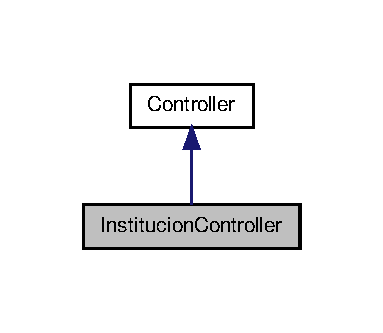
\includegraphics[width=184pt]{class_app_1_1_http_1_1_controllers_1_1_institucion_controller__inherit__graph}
\end{center}
\end{figure}


\-Diagrama de colaboración para \-Institucion\-Controller\-:
\nopagebreak
\begin{figure}[H]
\begin{center}
\leavevmode
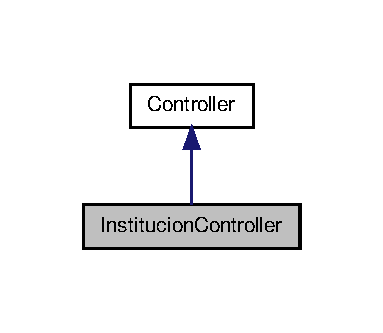
\includegraphics[width=184pt]{class_app_1_1_http_1_1_controllers_1_1_institucion_controller__coll__graph}
\end{center}
\end{figure}
\subsection*{\-Métodos públicos}
\begin{DoxyCompactItemize}
\item 
\hyperlink{class_app_1_1_http_1_1_controllers_1_1_institucion_controller_a621841b235a1cc220b5e4f52e458899c}{index} (\$institucion)
\item 
\hyperlink{class_app_1_1_http_1_1_controllers_1_1_institucion_controller_ae7e2d05cf98cc9ae1dced18d7778355b}{ver\-Aviso} (\$institucion, \$aviso)
\end{DoxyCompactItemize}


\subsection{\-Documentación de las funciones miembro}
\hypertarget{class_app_1_1_http_1_1_controllers_1_1_institucion_controller_a621841b235a1cc220b5e4f52e458899c}{\index{\-App\-::\-Http\-::\-Controllers\-::\-Institucion\-Controller@{\-App\-::\-Http\-::\-Controllers\-::\-Institucion\-Controller}!index@{index}}
\index{index@{index}!App::Http::Controllers::InstitucionController@{\-App\-::\-Http\-::\-Controllers\-::\-Institucion\-Controller}}
\subsubsection[{index}]{\setlength{\rightskip}{0pt plus 5cm}{\bf index} (
\begin{DoxyParamCaption}
\item[{\$}]{institucion}
\end{DoxyParamCaption}
)}}\label{class_app_1_1_http_1_1_controllers_1_1_institucion_controller_a621841b235a1cc220b5e4f52e458899c}
\-Recibe petición \-G\-E\-T a '/institucion/\{institucion?\}' \-Retorna la vista con toda la información de la institución solicitada


\begin{DoxyParams}{\-Parámetros}
{\em $<$type$>$} & \$institucion \-El nombre de la institución solicitada\\
\hline
\end{DoxyParams}
\begin{DoxyReturn}{\-Devuelve}
$<$type$>$ ( description\-\_\-of\-\_\-the\-\_\-return\-\_\-value ) 
\end{DoxyReturn}
\hypertarget{class_app_1_1_http_1_1_controllers_1_1_institucion_controller_ae7e2d05cf98cc9ae1dced18d7778355b}{\index{\-App\-::\-Http\-::\-Controllers\-::\-Institucion\-Controller@{\-App\-::\-Http\-::\-Controllers\-::\-Institucion\-Controller}!ver\-Aviso@{ver\-Aviso}}
\index{ver\-Aviso@{ver\-Aviso}!App::Http::Controllers::InstitucionController@{\-App\-::\-Http\-::\-Controllers\-::\-Institucion\-Controller}}
\subsubsection[{ver\-Aviso}]{\setlength{\rightskip}{0pt plus 5cm}{\bf ver\-Aviso} (
\begin{DoxyParamCaption}
\item[{\$}]{institucion, }
\item[{\$}]{aviso}
\end{DoxyParamCaption}
)}}\label{class_app_1_1_http_1_1_controllers_1_1_institucion_controller_ae7e2d05cf98cc9ae1dced18d7778355b}
\-Recibe petición \-G\-E\-T a '/institucion/\{institucion?\}/aviso/\{aviso?\}' \-Busca el aviso y si es que este pertenece a la institución que se pide \-Si está bien. retorna la vista que muestra información del aviso solicitado \-Sino, retorna una vista de error (por ahora)


\begin{DoxyParams}{\-Parámetros}
{\em $<$type$>$} & \$institucion \-The institucion \\
\hline
{\em $<$type$>$} & \$aviso \-The aviso\\
\hline
\end{DoxyParams}
\begin{DoxyReturn}{\-Devuelve}
$<$type$>$ ( description\-\_\-of\-\_\-the\-\_\-return\-\_\-value ) 
\end{DoxyReturn}


\-La documentación para esta clase fue generada a partir del siguiente fichero\-:\begin{DoxyCompactItemize}
\item 
/home/travis/build/tvargasvicencio/ayudalab/app/\-Http/\-Controllers/\-Institucion\-Controller.\-php\end{DoxyCompactItemize}

\hypertarget{class_institucion_table_seeder}{\section{\-Referencia de la \-Clase \-Institucion\-Table\-Seeder}
\label{class_institucion_table_seeder}\index{\-Institucion\-Table\-Seeder@{\-Institucion\-Table\-Seeder}}
}
\subsection*{\-Métodos públicos}
\begin{DoxyCompactItemize}
\item 
\hyperlink{class_institucion_table_seeder_afb0fafe7e02a3ae1993c01c19fad2bae}{run} ()
\end{DoxyCompactItemize}


\subsection{\-Documentación de las funciones miembro}
\hypertarget{class_institucion_table_seeder_afb0fafe7e02a3ae1993c01c19fad2bae}{\index{\-Institucion\-Table\-Seeder@{\-Institucion\-Table\-Seeder}!run@{run}}
\index{run@{run}!InstitucionTableSeeder@{\-Institucion\-Table\-Seeder}}
\subsubsection[{run}]{\setlength{\rightskip}{0pt plus 5cm}{\bf run} (
\begin{DoxyParamCaption}
{}
\end{DoxyParamCaption}
)}}\label{class_institucion_table_seeder_afb0fafe7e02a3ae1993c01c19fad2bae}
\-Run the database seeds.

\begin{DoxyReturn}{\-Devuelve}
void 
\end{DoxyReturn}


\-La documentación para esta clase fue generada a partir del siguiente fichero\-:\begin{DoxyCompactItemize}
\item 
/home/travis/build/tvargasvicencio/ayudalab/database/seeds/\-Institucion\-Table\-Seeder.\-php\end{DoxyCompactItemize}

\hypertarget{class_app_1_1_noticia}{\section{\-Referencia de la \-Clase \-Noticia}
\label{class_app_1_1_noticia}\index{\-Noticia@{\-Noticia}}
}
\subsection*{\-Métodos públicos}
\begin{DoxyCompactItemize}
\item 
\hyperlink{class_app_1_1_noticia_abfb0e179daf0a8f710adbb1456e5b3eb}{institucion} ()
\item 
\hyperlink{class_app_1_1_noticia_ae8a275690ff1b618e1947378b0ed73ae}{user} ()
\item 
\hypertarget{class_app_1_1_noticia_aab357d399e9c51ed8c88f378bf1b9d05}{{\bfseries imagenes} ()}\label{class_app_1_1_noticia_aab357d399e9c51ed8c88f378bf1b9d05}

\end{DoxyCompactItemize}
\subsection*{\-Atributos protegidos}
\begin{DoxyCompactItemize}
\item 
\hypertarget{class_app_1_1_noticia_ae8876a14058f368335baccf35af4a22b}{{\bfseries \$table} = 'noticia'}\label{class_app_1_1_noticia_ae8876a14058f368335baccf35af4a22b}

\item 
\hypertarget{class_app_1_1_noticia_a6a90e74ccdf5efd70d51d10c906f8e32}{{\bfseries \$fillable} = \mbox{[}'descripcion', 'titulo', 'rut\-\_\-inst', 'user\-\_\-id'\mbox{]}}\label{class_app_1_1_noticia_a6a90e74ccdf5efd70d51d10c906f8e32}

\end{DoxyCompactItemize}


\subsection{\-Documentación de las funciones miembro}
\hypertarget{class_app_1_1_noticia_abfb0e179daf0a8f710adbb1456e5b3eb}{\index{\-App\-::\-Noticia@{\-App\-::\-Noticia}!institucion@{institucion}}
\index{institucion@{institucion}!App::Noticia@{\-App\-::\-Noticia}}
\subsubsection[{institucion}]{\setlength{\rightskip}{0pt plus 5cm}{\bf institucion} (
\begin{DoxyParamCaption}
{}
\end{DoxyParamCaption}
)}}\label{class_app_1_1_noticia_abfb0e179daf0a8f710adbb1456e5b3eb}
\-Indica que un \hyperlink{class_app_1_1_aviso}{\-Aviso} pertenece a una \hyperlink{class_app_1_1_institucion}{\-Institucion}

\begin{DoxyReturn}{\-Devuelve}
$<$type$>$ ( description\-\_\-of\-\_\-the\-\_\-return\-\_\-value ) 
\end{DoxyReturn}
\hypertarget{class_app_1_1_noticia_ae8a275690ff1b618e1947378b0ed73ae}{\index{\-App\-::\-Noticia@{\-App\-::\-Noticia}!user@{user}}
\index{user@{user}!App::Noticia@{\-App\-::\-Noticia}}
\subsubsection[{user}]{\setlength{\rightskip}{0pt plus 5cm}{\bf user} (
\begin{DoxyParamCaption}
{}
\end{DoxyParamCaption}
)}}\label{class_app_1_1_noticia_ae8a275690ff1b618e1947378b0ed73ae}
\-Indica que un \hyperlink{class_app_1_1_aviso}{\-Aviso} pertenece a un \hyperlink{class_app_1_1_user}{\-User}

\begin{DoxyReturn}{\-Devuelve}
$<$type$>$ ( description\-\_\-of\-\_\-the\-\_\-return\-\_\-value ) 
\end{DoxyReturn}


\-La documentación para esta clase fue generada a partir del siguiente fichero\-:\begin{DoxyCompactItemize}
\item 
/home/travis/build/tvargasvicencio/ayudalab/app/\-Noticia.\-php\end{DoxyCompactItemize}

\hypertarget{class_app_1_1_http_1_1_controllers_1_1_auth_1_1_password_controller}{\section{\-Referencia de la \-Clase \-Password\-Controller}
\label{class_app_1_1_http_1_1_controllers_1_1_auth_1_1_password_controller}\index{\-Password\-Controller@{\-Password\-Controller}}
}


\-Diagrama de herencias de \-Password\-Controller
\nopagebreak
\begin{figure}[H]
\begin{center}
\leavevmode
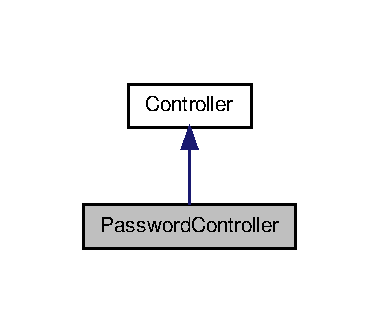
\includegraphics[width=182pt]{class_app_1_1_http_1_1_controllers_1_1_auth_1_1_password_controller__inherit__graph}
\end{center}
\end{figure}


\-Diagrama de colaboración para \-Password\-Controller\-:
\nopagebreak
\begin{figure}[H]
\begin{center}
\leavevmode
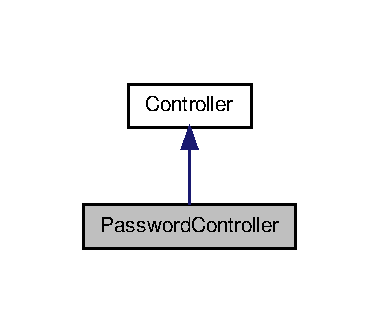
\includegraphics[width=182pt]{class_app_1_1_http_1_1_controllers_1_1_auth_1_1_password_controller__coll__graph}
\end{center}
\end{figure}
\subsection*{\-Métodos públicos}
\begin{DoxyCompactItemize}
\item 
\hyperlink{class_app_1_1_http_1_1_controllers_1_1_auth_1_1_password_controller_a095c5d389db211932136b53f25f39685}{\-\_\-\-\_\-construct} ()
\end{DoxyCompactItemize}


\subsection{\-Documentación del constructor y destructor}
\hypertarget{class_app_1_1_http_1_1_controllers_1_1_auth_1_1_password_controller_a095c5d389db211932136b53f25f39685}{\index{\-App\-::\-Http\-::\-Controllers\-::\-Auth\-::\-Password\-Controller@{\-App\-::\-Http\-::\-Controllers\-::\-Auth\-::\-Password\-Controller}!\-\_\-\-\_\-construct@{\-\_\-\-\_\-construct}}
\index{\-\_\-\-\_\-construct@{\-\_\-\-\_\-construct}!App::Http::Controllers::Auth::PasswordController@{\-App\-::\-Http\-::\-Controllers\-::\-Auth\-::\-Password\-Controller}}
\subsubsection[{\-\_\-\-\_\-construct}]{\setlength{\rightskip}{0pt plus 5cm}{\bf \-\_\-\-\_\-construct} (
\begin{DoxyParamCaption}
{}
\end{DoxyParamCaption}
)}}\label{class_app_1_1_http_1_1_controllers_1_1_auth_1_1_password_controller_a095c5d389db211932136b53f25f39685}
\-Create a new password controller instance.

\begin{DoxyReturn}{\-Devuelve}
void 
\end{DoxyReturn}


\-La documentación para esta clase fue generada a partir del siguiente fichero\-:\begin{DoxyCompactItemize}
\item 
/home/travis/build/tvargasvicencio/ayudalab/app/\-Http/\-Controllers/\-Auth/\-Password\-Controller.\-php\end{DoxyCompactItemize}

\hypertarget{class_app_1_1_http_1_1_controllers_1_1_storage_controller}{\section{\-Referencia de la \-Clase \-Storage\-Controller}
\label{class_app_1_1_http_1_1_controllers_1_1_storage_controller}\index{\-Storage\-Controller@{\-Storage\-Controller}}
}


\-Diagrama de herencias de \-Storage\-Controller
\nopagebreak
\begin{figure}[H]
\begin{center}
\leavevmode
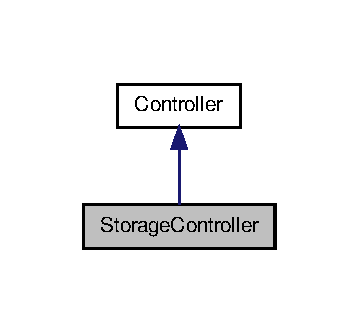
\includegraphics[width=172pt]{class_app_1_1_http_1_1_controllers_1_1_storage_controller__inherit__graph}
\end{center}
\end{figure}


\-Diagrama de colaboración para \-Storage\-Controller\-:
\nopagebreak
\begin{figure}[H]
\begin{center}
\leavevmode
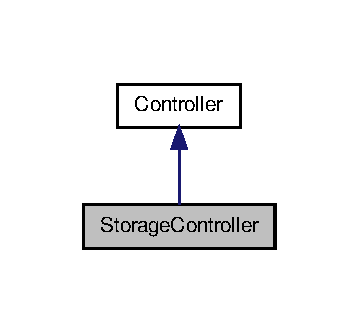
\includegraphics[width=172pt]{class_app_1_1_http_1_1_controllers_1_1_storage_controller__coll__graph}
\end{center}
\end{figure}
\subsection*{\-Métodos públicos}
\begin{DoxyCompactItemize}
\item 
\hypertarget{class_app_1_1_http_1_1_controllers_1_1_storage_controller_a149eb92716c1084a935e04a8d95f7347}{{\bfseries index} ()}\label{class_app_1_1_http_1_1_controllers_1_1_storage_controller_a149eb92716c1084a935e04a8d95f7347}

\item 
\hypertarget{class_app_1_1_http_1_1_controllers_1_1_storage_controller_a5369f058d8c1c480e4d4775b8bc0a633}{{\bfseries save} (\-Request \$r)}\label{class_app_1_1_http_1_1_controllers_1_1_storage_controller_a5369f058d8c1c480e4d4775b8bc0a633}

\item 
\hypertarget{class_app_1_1_http_1_1_controllers_1_1_storage_controller_a4208fb06ad4d1df850e52354c7c455b7}{{\bfseries mostrar\-Imagen} (\$id)}\label{class_app_1_1_http_1_1_controllers_1_1_storage_controller_a4208fb06ad4d1df850e52354c7c455b7}

\end{DoxyCompactItemize}


\-La documentación para esta clase fue generada a partir del siguiente fichero\-:\begin{DoxyCompactItemize}
\item 
/home/travis/build/tvargasvicencio/ayudalab/app/\-Http/\-Controllers/\-Storage\-Controller.\-php\end{DoxyCompactItemize}

\hypertarget{class_tabla_imagen}{\section{\-Referencia de la \-Clase \-Tabla\-Imagen}
\label{class_tabla_imagen}\index{\-Tabla\-Imagen@{\-Tabla\-Imagen}}
}
\subsection*{\-Métodos públicos}
\begin{DoxyCompactItemize}
\item 
\hyperlink{class_tabla_imagen_a4edef5efd5ab94ce9d17295898ead93a}{up} ()
\item 
\hyperlink{class_tabla_imagen_af5fda92f47a449c7a33f9dd5ef5aa6c3}{down} ()
\end{DoxyCompactItemize}


\subsection{\-Documentación de las funciones miembro}
\hypertarget{class_tabla_imagen_af5fda92f47a449c7a33f9dd5ef5aa6c3}{\index{\-Tabla\-Imagen@{\-Tabla\-Imagen}!down@{down}}
\index{down@{down}!TablaImagen@{\-Tabla\-Imagen}}
\subsubsection[{down}]{\setlength{\rightskip}{0pt plus 5cm}{\bf down} (
\begin{DoxyParamCaption}
{}
\end{DoxyParamCaption}
)}}\label{class_tabla_imagen_af5fda92f47a449c7a33f9dd5ef5aa6c3}
\-Reverse the migrations.

\begin{DoxyReturn}{\-Devuelve}
void 
\end{DoxyReturn}
\hypertarget{class_tabla_imagen_a4edef5efd5ab94ce9d17295898ead93a}{\index{\-Tabla\-Imagen@{\-Tabla\-Imagen}!up@{up}}
\index{up@{up}!TablaImagen@{\-Tabla\-Imagen}}
\subsubsection[{up}]{\setlength{\rightskip}{0pt plus 5cm}{\bf up} (
\begin{DoxyParamCaption}
{}
\end{DoxyParamCaption}
)}}\label{class_tabla_imagen_a4edef5efd5ab94ce9d17295898ead93a}
\-Run the migrations.

\begin{DoxyReturn}{\-Devuelve}
void 
\end{DoxyReturn}


\-La documentación para esta clase fue generada a partir del siguiente fichero\-:\begin{DoxyCompactItemize}
\item 
/home/travis/build/tvargasvicencio/ayudalab/database/migrations/2017\-\_\-04\-\_\-11\-\_\-032423\-\_\-tabla\-\_\-imagen.\-php\end{DoxyCompactItemize}

\hypertarget{class_tabla_imagen_evento}{\section{\-Referencia de la \-Clase \-Tabla\-Imagen\-Evento}
\label{class_tabla_imagen_evento}\index{\-Tabla\-Imagen\-Evento@{\-Tabla\-Imagen\-Evento}}
}
\subsection*{\-Métodos públicos}
\begin{DoxyCompactItemize}
\item 
\hyperlink{class_tabla_imagen_evento_a4edef5efd5ab94ce9d17295898ead93a}{up} ()
\item 
\hyperlink{class_tabla_imagen_evento_af5fda92f47a449c7a33f9dd5ef5aa6c3}{down} ()
\end{DoxyCompactItemize}


\subsection{\-Documentación de las funciones miembro}
\hypertarget{class_tabla_imagen_evento_af5fda92f47a449c7a33f9dd5ef5aa6c3}{\index{\-Tabla\-Imagen\-Evento@{\-Tabla\-Imagen\-Evento}!down@{down}}
\index{down@{down}!TablaImagenEvento@{\-Tabla\-Imagen\-Evento}}
\subsubsection[{down}]{\setlength{\rightskip}{0pt plus 5cm}{\bf down} (
\begin{DoxyParamCaption}
{}
\end{DoxyParamCaption}
)}}\label{class_tabla_imagen_evento_af5fda92f47a449c7a33f9dd5ef5aa6c3}
\-Reverse the migrations.

\begin{DoxyReturn}{\-Devuelve}
void 
\end{DoxyReturn}
\hypertarget{class_tabla_imagen_evento_a4edef5efd5ab94ce9d17295898ead93a}{\index{\-Tabla\-Imagen\-Evento@{\-Tabla\-Imagen\-Evento}!up@{up}}
\index{up@{up}!TablaImagenEvento@{\-Tabla\-Imagen\-Evento}}
\subsubsection[{up}]{\setlength{\rightskip}{0pt plus 5cm}{\bf up} (
\begin{DoxyParamCaption}
{}
\end{DoxyParamCaption}
)}}\label{class_tabla_imagen_evento_a4edef5efd5ab94ce9d17295898ead93a}
\-Run the migrations.

\begin{DoxyReturn}{\-Devuelve}
void 
\end{DoxyReturn}


\-La documentación para esta clase fue generada a partir del siguiente fichero\-:\begin{DoxyCompactItemize}
\item 
/home/travis/build/tvargasvicencio/ayudalab/database/migrations/2017\-\_\-04\-\_\-12\-\_\-195824\-\_\-tabla\-\_\-imagen\-\_\-evento.\-php\end{DoxyCompactItemize}

\hypertarget{class_tabla_noticia}{\section{\-Referencia de la \-Clase \-Tabla\-Noticia}
\label{class_tabla_noticia}\index{\-Tabla\-Noticia@{\-Tabla\-Noticia}}
}
\subsection*{\-Métodos públicos}
\begin{DoxyCompactItemize}
\item 
\hyperlink{class_tabla_noticia_a4edef5efd5ab94ce9d17295898ead93a}{up} ()
\item 
\hyperlink{class_tabla_noticia_af5fda92f47a449c7a33f9dd5ef5aa6c3}{down} ()
\end{DoxyCompactItemize}


\subsection{\-Documentación de las funciones miembro}
\hypertarget{class_tabla_noticia_af5fda92f47a449c7a33f9dd5ef5aa6c3}{\index{\-Tabla\-Noticia@{\-Tabla\-Noticia}!down@{down}}
\index{down@{down}!TablaNoticia@{\-Tabla\-Noticia}}
\subsubsection[{down}]{\setlength{\rightskip}{0pt plus 5cm}{\bf down} (
\begin{DoxyParamCaption}
{}
\end{DoxyParamCaption}
)}}\label{class_tabla_noticia_af5fda92f47a449c7a33f9dd5ef5aa6c3}
\-Reverse the migrations.

\begin{DoxyReturn}{\-Devuelve}
void 
\end{DoxyReturn}
\hypertarget{class_tabla_noticia_a4edef5efd5ab94ce9d17295898ead93a}{\index{\-Tabla\-Noticia@{\-Tabla\-Noticia}!up@{up}}
\index{up@{up}!TablaNoticia@{\-Tabla\-Noticia}}
\subsubsection[{up}]{\setlength{\rightskip}{0pt plus 5cm}{\bf up} (
\begin{DoxyParamCaption}
{}
\end{DoxyParamCaption}
)}}\label{class_tabla_noticia_a4edef5efd5ab94ce9d17295898ead93a}
\-Run the migrations.

\begin{DoxyReturn}{\-Devuelve}
void 
\end{DoxyReturn}


\-La documentación para esta clase fue generada a partir del siguiente fichero\-:\begin{DoxyCompactItemize}
\item 
/home/travis/build/tvargasvicencio/ayudalab/database/migrations/2017\-\_\-04\-\_\-12\-\_\-183436\-\_\-tabla\-\_\-noticia.\-php\end{DoxyCompactItemize}

\hypertarget{class_test_case}{\section{\-Referencia de la \-Clase \-Test\-Case}
\label{class_test_case}\index{\-Test\-Case@{\-Test\-Case}}
}


\-Diagrama de herencias de \-Test\-Case
\nopagebreak
\begin{figure}[H]
\begin{center}
\leavevmode
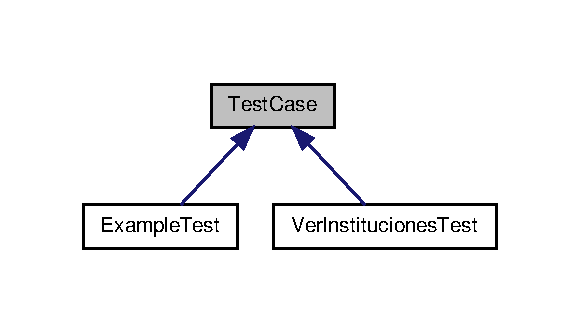
\includegraphics[width=278pt]{class_test_case__inherit__graph}
\end{center}
\end{figure}
\subsection*{\-Métodos públicos}
\begin{DoxyCompactItemize}
\item 
\hyperlink{class_test_case_ac39b08beb1abc87ef3f463b559d4c7fe}{create\-Application} ()
\end{DoxyCompactItemize}
\subsection*{\-Atributos protegidos}
\begin{DoxyCompactItemize}
\item 
\hypertarget{class_test_case_a3f46653370faceec6ea1f4999c3a9ca2}{{\bfseries \$base\-Url} = 'http\-://localhost'}\label{class_test_case_a3f46653370faceec6ea1f4999c3a9ca2}

\end{DoxyCompactItemize}


\subsection{\-Documentación de las funciones miembro}
\hypertarget{class_test_case_ac39b08beb1abc87ef3f463b559d4c7fe}{\index{\-Test\-Case@{\-Test\-Case}!create\-Application@{create\-Application}}
\index{create\-Application@{create\-Application}!TestCase@{\-Test\-Case}}
\subsubsection[{create\-Application}]{\setlength{\rightskip}{0pt plus 5cm}{\bf create\-Application} (
\begin{DoxyParamCaption}
{}
\end{DoxyParamCaption}
)}}\label{class_test_case_ac39b08beb1abc87ef3f463b559d4c7fe}
\-Creates the application.

\begin{DoxyReturn}{\-Devuelve}

\end{DoxyReturn}


\-La documentación para esta clase fue generada a partir del siguiente fichero\-:\begin{DoxyCompactItemize}
\item 
/home/travis/build/tvargasvicencio/ayudalab/tests/\-Test\-Case.\-php\end{DoxyCompactItemize}

\hypertarget{class_app_1_1_user}{\section{\-Referencia de la \-Clase \-User}
\label{class_app_1_1_user}\index{\-User@{\-User}}
}
\subsection*{\-Métodos públicos}
\begin{DoxyCompactItemize}
\item 
\hyperlink{class_app_1_1_user_a893f830558ee917f86dae4c21bc95319}{aviso} ()
\item 
\hyperlink{class_app_1_1_user_abfb0e179daf0a8f710adbb1456e5b3eb}{institucion} ()
\end{DoxyCompactItemize}
\subsection*{\-Atributos protegidos}
\begin{DoxyCompactItemize}
\item 
{\bfseries \$fillable}
\item 
{\bfseries \$hidden}
\end{DoxyCompactItemize}


\subsection{\-Documentación de las funciones miembro}
\hypertarget{class_app_1_1_user_a893f830558ee917f86dae4c21bc95319}{\index{\-App\-::\-User@{\-App\-::\-User}!aviso@{aviso}}
\index{aviso@{aviso}!App::User@{\-App\-::\-User}}
\subsubsection[{aviso}]{\setlength{\rightskip}{0pt plus 5cm}{\bf aviso} (
\begin{DoxyParamCaption}
{}
\end{DoxyParamCaption}
)}}\label{class_app_1_1_user_a893f830558ee917f86dae4c21bc95319}
\-Indica que \hyperlink{class_app_1_1_user}{\-User} puede tener muchos aviso

\begin{DoxyReturn}{\-Devuelve}
$<$type$>$ ( description\-\_\-of\-\_\-the\-\_\-return\-\_\-value ) 
\end{DoxyReturn}
\hypertarget{class_app_1_1_user_abfb0e179daf0a8f710adbb1456e5b3eb}{\index{\-App\-::\-User@{\-App\-::\-User}!institucion@{institucion}}
\index{institucion@{institucion}!App::User@{\-App\-::\-User}}
\subsubsection[{institucion}]{\setlength{\rightskip}{0pt plus 5cm}{\bf institucion} (
\begin{DoxyParamCaption}
{}
\end{DoxyParamCaption}
)}}\label{class_app_1_1_user_abfb0e179daf0a8f710adbb1456e5b3eb}
\-Indica que \hyperlink{class_app_1_1_user}{\-User} pertenece a una institucion

\begin{DoxyReturn}{\-Devuelve}
$<$type$>$ ( description\-\_\-of\-\_\-the\-\_\-return\-\_\-value ) 
\end{DoxyReturn}


\subsection{\-Documentación de los campos}
\hypertarget{class_app_1_1_user_a6a90e74ccdf5efd70d51d10c906f8e32}{\index{\-App\-::\-User@{\-App\-::\-User}!\$fillable@{\$fillable}}
\index{\$fillable@{\$fillable}!App::User@{\-App\-::\-User}}
\subsubsection[{\$fillable}]{\setlength{\rightskip}{0pt plus 5cm}\$fillable\hspace{0.3cm}{\ttfamily  \mbox{[}protected\mbox{]}}}}\label{class_app_1_1_user_a6a90e74ccdf5efd70d51d10c906f8e32}
{\bfseries \-Valor inicial\-:}
\begin{DoxyCode}
 [
        'name', 'email', 'password', 'rut_inst'
    ]
\end{DoxyCode}
\hypertarget{class_app_1_1_user_a4a374564d2858d8ae869a8fb890aad56}{\index{\-App\-::\-User@{\-App\-::\-User}!\$hidden@{\$hidden}}
\index{\$hidden@{\$hidden}!App::User@{\-App\-::\-User}}
\subsubsection[{\$hidden}]{\setlength{\rightskip}{0pt plus 5cm}\$hidden\hspace{0.3cm}{\ttfamily  \mbox{[}protected\mbox{]}}}}\label{class_app_1_1_user_a4a374564d2858d8ae869a8fb890aad56}
{\bfseries \-Valor inicial\-:}
\begin{DoxyCode}
 [
        'password', 'remember_token',
    ]
\end{DoxyCode}


\-La documentación para esta clase fue generada a partir del siguiente fichero\-:\begin{DoxyCompactItemize}
\item 
/home/travis/build/tvargasvicencio/ayudalab/app/\-User.\-php\end{DoxyCompactItemize}

\hypertarget{class_user_table_seeder}{\section{\-Referencia de la \-Clase \-User\-Table\-Seeder}
\label{class_user_table_seeder}\index{\-User\-Table\-Seeder@{\-User\-Table\-Seeder}}
}
\subsection*{\-Métodos públicos}
\begin{DoxyCompactItemize}
\item 
\hyperlink{class_user_table_seeder_afb0fafe7e02a3ae1993c01c19fad2bae}{run} ()
\end{DoxyCompactItemize}


\subsection{\-Documentación de las funciones miembro}
\hypertarget{class_user_table_seeder_afb0fafe7e02a3ae1993c01c19fad2bae}{\index{\-User\-Table\-Seeder@{\-User\-Table\-Seeder}!run@{run}}
\index{run@{run}!UserTableSeeder@{\-User\-Table\-Seeder}}
\subsubsection[{run}]{\setlength{\rightskip}{0pt plus 5cm}{\bf run} (
\begin{DoxyParamCaption}
{}
\end{DoxyParamCaption}
)}}\label{class_user_table_seeder_afb0fafe7e02a3ae1993c01c19fad2bae}
\-Run the database seeds.

\begin{DoxyReturn}{\-Devuelve}
void 
\end{DoxyReturn}


\-La documentación para esta clase fue generada a partir del siguiente fichero\-:\begin{DoxyCompactItemize}
\item 
/home/travis/build/tvargasvicencio/ayudalab/database/seeds/\-User\-Table\-Seeder.\-php\end{DoxyCompactItemize}

\hypertarget{class_ver_instituciones_test}{\section{\-Referencia de la \-Clase \-Ver\-Instituciones\-Test}
\label{class_ver_instituciones_test}\index{\-Ver\-Instituciones\-Test@{\-Ver\-Instituciones\-Test}}
}


\-Diagrama de herencias de \-Ver\-Instituciones\-Test
\nopagebreak
\begin{figure}[H]
\begin{center}
\leavevmode
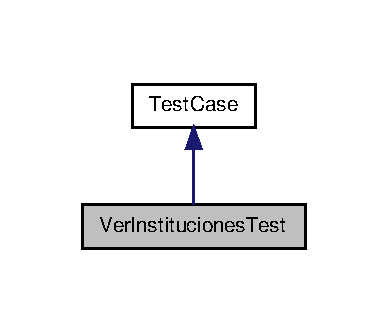
\includegraphics[width=186pt]{class_ver_instituciones_test__inherit__graph}
\end{center}
\end{figure}


\-Diagrama de colaboración para \-Ver\-Instituciones\-Test\-:
\nopagebreak
\begin{figure}[H]
\begin{center}
\leavevmode
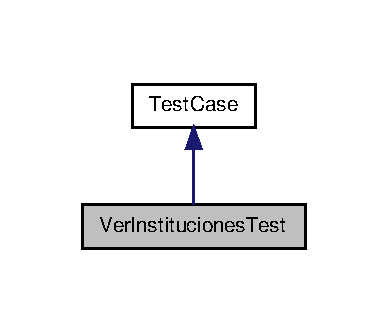
\includegraphics[width=186pt]{class_ver_instituciones_test__coll__graph}
\end{center}
\end{figure}
\subsection*{\-Métodos públicos}
\begin{DoxyCompactItemize}
\item 
\hyperlink{class_ver_instituciones_test_ac55dde95bf19a1ace1ae3caf3d8d2627}{test\-San\-Antonio} ()
\end{DoxyCompactItemize}


\subsection{\-Documentación de las funciones miembro}
\hypertarget{class_ver_instituciones_test_ac55dde95bf19a1ace1ae3caf3d8d2627}{\index{\-Ver\-Instituciones\-Test@{\-Ver\-Instituciones\-Test}!test\-San\-Antonio@{test\-San\-Antonio}}
\index{test\-San\-Antonio@{test\-San\-Antonio}!VerInstitucionesTest@{\-Ver\-Instituciones\-Test}}
\subsubsection[{test\-San\-Antonio}]{\setlength{\rightskip}{0pt plus 5cm}{\bf test\-San\-Antonio} (
\begin{DoxyParamCaption}
{}
\end{DoxyParamCaption}
)}}\label{class_ver_instituciones_test_ac55dde95bf19a1ace1ae3caf3d8d2627}
\-A basic test example.

\begin{DoxyReturn}{\-Devuelve}
void 
\end{DoxyReturn}


\-La documentación para esta clase fue generada a partir del siguiente fichero\-:\begin{DoxyCompactItemize}
\item 
/home/travis/build/tvargasvicencio/ayudalab/tests/\-Ver\-Instituciones\-Test.\-php\end{DoxyCompactItemize}

\printindex
\end{document}
